\section{Toạ độ vectơ}
\subsection{LÝ THUYẾT CẦN NHỚ}
\subsubsection{Trục tọa độ}
\indam{Định nghĩa:}
\begin{boxdn}
	\immini{\textbf{Trục tọa độ} (gọi tắt là \textbf{trục}) là một đường thẳng trên đó đã xác định một điểm $O$ (gọi là \textbf{điểm gốc}) và một vectơ $\overrightarrow{e}$ có độ dài bằng $1$ gọi là vectơ đơn vị của trục.\\
		Ta kí hiệu trục đó là $(O;\overrightarrow{e})$.}{\begin{tikzpicture}[scale=1, font=\footnotesize, line join=round, line cap=round, >=stealth]
			\draw (-1,0)--(4,0);
			\draw[->,red] (0,0)--(1,0) node[above,midway,rotate=0,black] {\footnotesize $\overrightarrow{e}$};
			\fill (0,0)circle(1.5pt)node[below] {\footnotesize $O$};
	\end{tikzpicture}}
\end{boxdn}
\subsubsection{Hệ trục tọa độ}
\indam{Định nghĩa:}
\begin{boxdn}
	\immini{\textbf{Hệ trục tọa độ} $\left( O;\overrightarrow{i},\overrightarrow{j}\right) $ gồm hai trục $\left( O;\overrightarrow{i}\right) $ và $\left( O;\overrightarrow{j}\right) $ vuông góc với nhau. Điểm gốc $O$ chung của hai trục gọi là \textbf{gốc tọa độ}. Trục $\left( O;\overrightarrow{i}\right) $ được gọi là \textbf{trục hoành} và kí hiệu là $Ox$, trục $\left( O;\overrightarrow{j}\right) $ được gọi là \textbf{trục tung} và kí hiệu là $Oy$. Các vectơ $\overrightarrow{i}$ và $\overrightarrow{j}$ là các vectơ đơn vị trên $Ox$ và $Oy$. Hệ trục toạ độ $\left( O;\overrightarrow{i},\overrightarrow{j}\right) $ còn được kí hiệu là $Oxy$.}{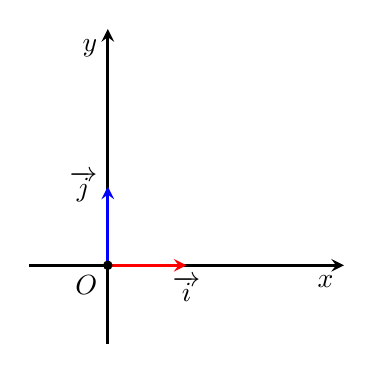
\begin{tikzpicture}[>=stealth,x=1cm,y=1cm]
			%\draw[line width=0.2pt] (-1,-1) grid (3,3);
			\draw[->,line width = 1pt] (-1,0)--(0,0)%
			node[below left]{$O$}--(1,0)--(3,0) node[below left]{$x$};
			\draw[->,line width = 1pt] (0,-1)--(0,1)--(0,3) node[below left]{$y$};
			\draw[->,line width = 1pt,red] (0,0) --(1,0) node[below,black]{$\overrightarrow{i}$};
			\draw[->,line width = 1pt,blue] (0,0) --(0,1) node[left,black]{$\overrightarrow{j}$};
			\draw[fill] (0,0) circle(1.5pt);
	\end{tikzpicture}}
\end{boxdn}
\begin{luuy}
	Mặt phẳng mà trên đó đã cho một hệ trục toạ độ $Oxy$ được gọi là mặt phẳng tọa độ $Oxy$, hay gọi tắt là mặt phẳng $Oxy$.
\end{luuy}

\subsubsection{Tọa độ của một vectơ}
\indam{Định nghĩa:}
\begin{boxdn}%[Tex hóa SGK CD-CT,T8/22, Đỗ Minh Phúc]%
	Trong mặt phẳng $Oxy$, cặp số $(x;y)$ trong biểu diễn $\overrightarrow{a}=x \overrightarrow{i}+y \overrightarrow{j}$ được gọi là \textbf{tọa độ} của vectơ $\overrightarrow{a}$, kí hiệu $\overrightarrow{a}=(x;y),$ $x$ gọi là \textbf{hoành độ}, $y$ gọi là \textbf{tung độ} của vectơ $\overrightarrow{a}$.
\end{boxdn}
\begin{luuy}
	\begin{itemize}
		\item $\overrightarrow{a}=(x ; y) \Leftrightarrow \overrightarrow{a}=x \overrightarrow{i}+y \overrightarrow{j}$.
		\item Nếu cho $\overrightarrow{a}=(x;y)$ và $\overrightarrow{b}=\left(x';y'\right)$ thì $\overrightarrow{a}=\overrightarrow{b} \Leftrightarrow\heva{&x=x' \\& y=y'.}$
	\end{itemize}
\end{luuy}

\subsubsection{Tọa độ của một điểm}
\indam{Định nghĩa:}
\immini{\begin{boxdn}
		Trong mặt phẳng toạ độ, cho một điểm $M$ tuỳ ý. Toạ độ của vectơ $\overrightarrow{OM}$ được gọi là \textbf{tọa độ} của điểm $M$.
\end{boxdn}}{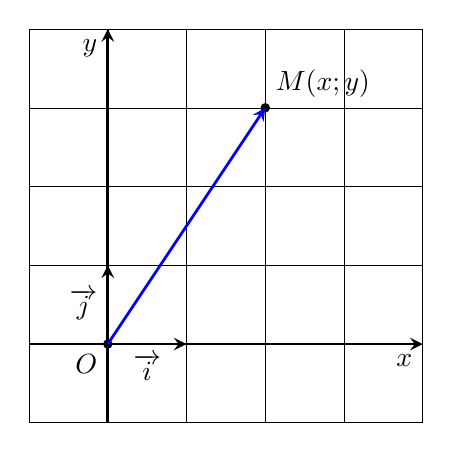
\begin{tikzpicture}[>=stealth,x=1cm,y=1cm]
		\draw[line width=0.2pt] (-1,-1) grid (4,4);
		\draw[->,line width = 1pt] (-1,0)--(0,0)%
		node[below left]{$O$}--(4,0) node[below left]{$x$};
		\draw[->,line width = 1pt] (0,-1)--(0,4) node[below left]{$y$};
		\draw[->,line width = 1pt] (0,0) --(1,0) node[below,midway,rotate=0]{$\overrightarrow{i}$};
		\draw[->,line width = 1pt] (0,0) --(0,1) node[left,midway,rotate=0]{$\overrightarrow{j}$};
		\draw[fill] (0,0) circle(1.5pt);
		\draw[fill] (2,3) circle(1.5pt);
		\draw[->,line width = 1pt,blue] (0,0) --(2,3) node[above right,black]{$M(x;y)$};
\end{tikzpicture}}

\begin{luuy}
	\begin{itemize}
		\item Nếu $\overrightarrow{O M}=(x;y)$ thì cặp số $(x;y)$ là toạ độ của điểm $M$, kí hiệu $M(x;y)$, $x$ gọi là \textbf{hoành độ}, $y$ gọi là \textbf{tung độ} của điểm $M$.
		\item $M(x;y) \Leftrightarrow \overrightarrow{OM}=x\overrightarrow{i}+y\overrightarrow{j}$.
		\item Hoành độ của điểm $M$ còn được kí hiệu là $x_{M}$, tung độ của điểm $M$ còn được kí hiệu là $y_{M}$. Khi đó ta viết $M\left(x_{M};y_{M}\right)$.
	\end{itemize}
\end{luuy}
\subsubsection{Biểu thức tọa độ của các phép toán vectơ}
\indam{Định lý:}
\begin{boxdn}
	Cho hai vectơ $\overrightarrow{a}=\left(a_{1} ; a_{2}\right)$, $\overrightarrow{b}=\left(b_{1} ; b_{2}\right)$ và số thực $k$. Khi đó:
	\begin{itemize}
		\item $\overrightarrow{a}+\overrightarrow{b}=\left(a_{1}+b_{1} ; a_{2}+b_{2}\right)$
		\item $\overrightarrow{a}-\overrightarrow{b}=\left(a_{1}-b_{1} ; a_{2}-b_{2}\right)$
		\item $k \overrightarrow{a}=\left(k a_{1} ; k a_{2}\right)$
		\item $\overrightarrow{a} \cdot \overrightarrow{b}=a_{1} b_{1}+a_{2} b_{2}$
	\end{itemize}
\end{boxdn}
\subsubsection{Liên hệ giữa toạ độ của điểm và toạ độ của vectơ trong mặt phẳng}
\indam{Định lý:}
\begin{boxdn}
	Cho hai điểm $A\left(x_{A} ; y_{A}\right)$, $B\left(x_{B} ; y_{B}\right)$. Ta có:
	$$\overrightarrow{AB}=\left(x_{B}-x_{A} ; y_{B}-y_{A}\right) .$$
\end{boxdn}
\subsubsection{Toạ độ trung điểm của đoạn thẳng và trọng tâm của tam giác}
\indam{Định lý:}
\begin{boxdn}
	Cho hai điểm $A\left(x_{A};y_{A}\right)$ và $B\left(x_{B};y_{B}\right)$. Toạ độ trung điểm $M\left(x_{M};y_{M}\right)$ của đoạn thẳng $AB$ là:
	$$x_{M}=\dfrac{x_{A}+x_{B}}{2},\ y_{M}=\dfrac{y_{A}+y_{B}}{2}.$$
	Cho tam giác $ABC$ có $A\left(x_{A};y_{A}\right)$, $B\left(x_{B};y_{B}\right)$, $C\left(x_{C};y_{C}\right)$. Toạ độ trọng tâm $G\left(x_{G};y_{G}\right)$ của tam giác $ABC$ là:
	$$x_{G}=\dfrac{x_{A}+x_{B}+x_{C}}{3},\ y_{G}=\dfrac{y_{A}+y_{B}+y_{C}}{3}.$$
\end{boxdn}
\subsubsection{Ứng dụng biểu thức toạ độ của các phép toán vectơ}
\indam{Định lý:}
\begin{boxdn}
	Cho hai vectơ $\overrightarrow{a}=\left(a_{1} ; a_{2}\right)$, $\overrightarrow{b}=\left(b_{1} ; b_{2}\right)$ và hai điểm $A\left(x_{A} ; y_{A}\right)$, $B\left(x_{B} ; y_{B}\right)$. Ta có:
	\begin{itemize}
		\item $\overrightarrow{a} \perp \overrightarrow{b} \Leftrightarrow a_{1} b_{1}+a_{2} b_{2}=0$;
		\item $\overrightarrow{a}$ và $\overrightarrow{b}$ cùng phương $\Leftrightarrow a_{1} b_{2}-a_{2} b_{1}=0$;
		\item $\left| \overrightarrow{a}\right| =\sqrt{a_{1}^{2}+a_{2}^{2}}$;
		\item $A B=\sqrt{\left(x_{B}-x_{A}\right)^{2}+\left(y_{B}-y_{A}\right)^{2}}$;
		\item $\cos (\overrightarrow{a}, \overrightarrow{b})=\dfrac{\overrightarrow{a} \cdot \overrightarrow{b}}{\left| \overrightarrow{a}\right|  \cdot\left| \overrightarrow{b}\right| }=\dfrac{a_{1} b_{1}+a_{2} b_{2}}{\sqrt{a_{1}^{2}+a_{2}^{2}} \cdot \sqrt{b_{1}^{2}+b_{2}^{2}}}$ $\left( \overrightarrow{a}, \overrightarrow{b} \text{ khác } \overrightarrow{0}\right) $.
	\end{itemize}
\end{boxdn}
%-------------------------------------------------------------------------------------------------------------
\subsection{PHÂN LOẠI VÀ PHƯƠNG PHÁP GIẢI TOÁN}%mỗi dạng 3 ví dụ
\begin{dang}{Tìm tọa độ của vectơ, điểm dựa trên biểu thức tọa độ của các phép toán vectơ}
\textbf{Phương pháp giải}
\begin{itemize}
    \item Sử dụng các công thức tọa độ của tổng, hiệu, tích một số với một vectơ:\\
    Cho $\vec{a}=(a_1; a_2)$, $\vec{b}=(b_1; b_2)$ và $k \in \mathbb{R}$:
    \begin{itemize}
        \item $\vec{a} \pm \vec{b} = (a_1 \pm b_1; a_2 \pm b_2)$
        \item $k\vec{a} = (ka_1; ka_2)$
    \end{itemize}
    \item Tọa độ của vectơ $\vec{AB}$ với $A(x_A; y_A)$, $B(x_B; y_B)$ là $\vec{AB} = (x_B - x_A; y_B - y_A)$.
    \item Từ một hệ thức vectơ cho trước, ta thay tọa độ của các vectơ thành phần và thực hiện tính toán trên từng thành phần (hoành độ theo hoành độ, tung độ theo tung độ) để tìm kết quả.
\end{itemize}
\end{dang}
\begin{vd}%[0H9H1-2]%Ví dụ 1
	Tìm tọa độ các vectơ sau
	\begin{listEX}[4]
		\item $\overrightarrow{a}=2\overrightarrow{i}+3\overrightarrow{j}$.
		\item $\overrightarrow{b}=-\overrightarrow{i}+2\overrightarrow{j}$.
		\item $\overrightarrow{c}=-5\overrightarrow{i}$.
		\item $\overrightarrow{d}=4\overrightarrow{j}$.
	\end{listEX}
	\loigiai
	{
		\begin{itemize}
			\item[a)] Ta có $\overrightarrow{a}=2\overrightarrow{i}+3\overrightarrow{j} \Leftrightarrow \overrightarrow{a}=(2;3)$.
			\item[b)] Ta có $\overrightarrow{b}=-\overrightarrow{i}+2\overrightarrow{j} \Leftrightarrow \overrightarrow{b}=(-1;2)$.
			\item[c)] Ta có $\overrightarrow{c}=-5\overrightarrow{i} \Leftrightarrow \overrightarrow{c}=(-5;0)$.
			\item[d)] Ta có $\overrightarrow{d}=4\overrightarrow{j} \Leftrightarrow \overrightarrow{d}=(0;4)$.
		\end{itemize}
	}
\end{vd}
\begin{vd}[Sách bài tập CTST]%[0H9H1-2]
	Cho ba vectơ $\overrightarrow{m}=(-6;1)$, $\overrightarrow{n}=(0;2)$, $\overrightarrow{p}=(1;1)$. Tìm toạ độ của các vectơ
	\begin{enumerate}
		\item  $\overrightarrow{m}+\overrightarrow{n}-\overrightarrow{p}$.
		\item $(\overrightarrow{m} \cdot \overrightarrow{n})\overrightarrow{p}$.
	\end{enumerate}
	\loigiai{
		\begin{enumerate}
			\item Ta có: $\overrightarrow{m}+\overrightarrow{n}-\overrightarrow{p}=(-6+0-1;1+2-1)=(-7;2)$.
			\item Ta có: $(\overrightarrow{m} \cdot \overrightarrow{n})\overrightarrow{p}=(-6 \cdot 0+1 \cdot 2)\overrightarrow{p}=2\overrightarrow{p}=(2;2)$.
		\end{enumerate}
	}
\end{vd}
\begin{vd}%[0H9H1-3]
	Cho $A(2;-1)$, $B(-3;2)$, $C(-5;-2)$. Tìm tọa độ các vectơ $\overrightarrow{AB}$, $\overrightarrow{AC}$, $\overrightarrow{BC}$. 
	\loigiai{
		Ta có $\overrightarrow{AB}=(-5;3)$, $\overrightarrow{AC}=(-7;-1)$, $\overrightarrow{BC}=(-2;-4)$.
	}
\end{vd}
\begin{dang}
	{Tìm điều kiện để hai vectơ bằng nhau}
	\textbf{Phương pháp giải}
\begin{itemize}
    \item \textbf{Bước 1:} Tính tọa độ của hai vectơ $\vec{u} = (x_1; y_1)$ và $\vec{v} = (x_2; y_2)$ theo các tham số của bài toán.
    \item \textbf{Bước 2:} Áp dụng điều kiện hai vectơ bằng nhau:
    $$ \vec{u} = \vec{v} \Leftrightarrow \begin{cases} x_1 = x_2 \\ y_1 = y_2 \end{cases} $$
    \item \textbf{Bước 3:} Giải hệ phương trình trên để tìm giá trị của các tham số.
\end{itemize}
\end{dang}
\begin{vd}%[0H9H1-3]
	Tìm các số thực $a$ và $b$ sao cho mỗi cặp vectơ sau bằng nhau.
	\begin{enumerate}
		\item $\overrightarrow{m}=(3a-1;2b+1)$ và $\overrightarrow{n}=(-4;2)$;
		\item $\overrightarrow{u}=(2a-1;-3)$ và $\overrightarrow{v}=(3;4b+1)$;
		\item $\overrightarrow{x}=(a+b;-2a+3b)$ và $\overrightarrow{y}=(2a-3;4b)$.
	\end{enumerate}
	\loigiai{
		\begin{enumerate}
			\item $\overrightarrow{m}=\overrightarrow{n}\Leftrightarrow\heva{&3a-1=-4\\&2b+1=2}\Leftrightarrow\heva{&a=-1\\&b=\dfrac{1}{2}.}$
			\item $\overrightarrow{u}=\overrightarrow{v}\Leftrightarrow\heva{&2a-1=3\\&-3=4b+1}\Leftrightarrow\heva{&a=2\\&b=-1.}$
			\item $\overrightarrow{x}=\overrightarrow{y}\Leftrightarrow\heva{&a+b=2a-3\\&-2a+3b=4b}\Leftrightarrow\heva{&a-b=3\\&b=-2a}\Leftrightarrow\heva{&3a=3\\&b=-2a}\Leftrightarrow\heva{&a=1\\&b=-2.}$
		\end{enumerate}
	}
\end{vd}
\begin{vd}%[0H9H1-3]
	Trong mặt phẳng tọa độ $Oxy$, cho bốn điểm $A(-2;1)$, $B(2;3)$, $C(1;0)$, $D(-3;-2)$. Chứng minh $\overrightarrow{AB}=\overrightarrow{DC}$.
	\loigiai{
		Ta có: $\overrightarrow{AB}=(4;2)$, $\overrightarrow{DC}=(4;2)$. Suy ra $\overrightarrow{AB}=\overrightarrow{DC}$.
	}
\end{vd}
\begin{vd}%[0H9H1-3]
	Trong mặt phẳng $Oxy$, cho các điểm $A(-2;1)$, $B(4;0)$, $C(2;3)$. Tìm điểm $M$ biết rằng $\overrightarrow{CM}+3\overrightarrow{AC}=2\overrightarrow{AB}$.
	\loigiai{
		Gọi điểm $M(x;y)$. Khi đó ta có: $\overrightarrow{CM}=(x-2;y-3)$, $\overrightarrow{AC}=(4;2)$, $\overrightarrow{AB}=(6;-1)$.\\
		Theo giả thiết ta có $\overrightarrow{CM}+3\overrightarrow{AC}=2\overrightarrow{AB}\Leftrightarrow \heva{&x-2+3\cdot 4=2\cdot 6 \\&y-3+3\cdot 2=2\cdot (-1)}\Leftrightarrow \heva{&x=2 \\&y=-5.}$\\
		Vậy $M(2;-5)$.}
\end{vd}
\begin{dang}
	{Điều kiện để ba điểm thẳng hàng, hai vectơ cùng phương}
	\textbf{Phương pháp giải}
\begin{itemize}
    \item \textbf{Hai vectơ cùng phương:} Hai vectơ $\vec{u}=(x_1; y_1)$ và $\vec{v}=(x_2; y_2)$ cùng phương khi và chỉ khi có số thực $k$ sao cho $\vec{u}=k\vec{v}$. Biểu thức tọa độ tương đương là $x_1y_2 - x_2y_1 = 0$.
    \item \textbf{Ba điểm thẳng hàng:} Ba điểm $A, B, C$ phân biệt thẳng hàng khi và chỉ khi hai vectơ $\vec{AB}$ và $\vec{AC}$ cùng phương.
    \begin{enumerate}
        \item \textbf{Bước 1:} Tính tọa độ các vectơ $\vec{AB} = (x_B-x_A; y_B-y_A)$ và $\vec{AC} = (x_C-x_A; y_C-y_A)$.
        \item \textbf{Bước 2:} Áp dụng điều kiện cùng phương cho hai vectơ trên: $(x_B-x_A)(y_C-y_A) - (x_C-x_A)(y_B-y_A) = 0$.
    \end{enumerate}
\end{itemize}
\end{dang}
\begin{vd}%[0H9H1-4]
	\begin{itemize}
		\item[a)] Cho $\overrightarrow{u}=(2;-3)$, $\overrightarrow{v}=(2m-1;5)$. Tìm $m$ để $\overrightarrow{u}$ cùng phương $\overrightarrow{v}$.
		\item[b)] Cho $\overrightarrow{u}=(2;-5)$, $\overrightarrow{v}=(3;m)$. Tìm $m$ để $\overrightarrow{u}$ cùng phương $\overrightarrow{v}$.
		\item[c)] Cho $\overrightarrow{u}=(2x-3;-5)$, $\overrightarrow{v}=(3;5y+4)$. Tìm $x$, $y$ để $\overrightarrow{u} = \overrightarrow{v}$.
	\end{itemize}
	\loigiai
	{
		\begin{itemize}
			\item[a)] Để $\overrightarrow{u}$ cùng phương với $\overrightarrow{v}$ thì $2\cdot 5=-3\cdot (2m-1)\Leftrightarrow m=-\dfrac{7}{6}$.
			\item[b)] Để $\overrightarrow{u}$ cùng phương với $\overrightarrow{v}$ thì $2\cdot m=-5\cdot 3\Leftrightarrow m=-\dfrac{15}{2}$.
			\item[c)] Để $\overrightarrow{u} = \overrightarrow{v}$ thì $\heva{& 2x-3=3\\& -5=5y+4} \Leftrightarrow \heva{& x=3\\& y=-\dfrac{9}{5}.}$
		\end{itemize}
	}
\end{vd}
\begin{vd}%[0H9H1-4]
	\begin{enumerate}
		\item Cho $A(3;-2)$, $B(1;3)$. Tìm tọa độ điểm $M$ thuộc trục hoành sao cho $A$, $M$, $B$ thẳng hàng.
		\item Cho $A(3;-2)$, $B(1;3)$. Tìm tọa độ điểm $N$ thuộc trục tung sao cho $A$, $N$, $B$ thẳng hàng.
	\end{enumerate}
	\loigiai{
		\begin{enumerate}
			\item Do điểm $M$ thuộc trục hoành nên tọa độ điểm $M$ có dạng $(m;0)$.\\
			Ta có $A$, $M$, $B$ thẳng hàng nên tồn tại số $k$ để $\overrightarrow{AM}=k\overrightarrow{AB} \Rightarrow
			\heva {&m-3=-2k\\ &0+2=5k}\Leftrightarrow
			\heva {&m=-2\\ &k=\dfrac{5}{2}.}$\\
			Vậy $M(-2;0)$.
			\item Do điểm $N$ thuộc trục tung nên tọa độ điểm $N$ có dạng $(0;n)$.\\
			Ta có $A$, $N$, $B$ thẳng hàng nên tồn tại số $k$ để $\overrightarrow{AN}=k\overrightarrow{AB} \Rightarrow
			\heva {&0-3=-2k\\ &n+2=5k}\Leftrightarrow
			\heva {&n=13\\ &k=\dfrac{3}{2}.}$\\
			Vậy $N(0;13)$.
		\end{enumerate}
	}
\end{vd}

\begin{dang}
	{Tìm tọa độ trung điểm đoạn thẳng và tọa độ trọng tâm tam giác}
	\textbf{Phương pháp giải}
\begin{itemize}
    \item Tọa độ trung điểm $M$ của đoạn thẳng $AB$ được tính bằng công thức:
    $$ x_M = \frac{x_A+x_B}{2}; \quad y_M = \frac{y_A+y_B}{2} $$
    \item Tọa độ trọng tâm $G$ của tam giác $ABC$ được tính bằng công thức:
    $$ x_G = \frac{x_A+x_B+x_C}{3}; \quad y_G = \frac{y_A+y_B+y_C}{3} $$
    \item Tùy theo yêu cầu bài toán (tìm trung điểm/trọng tâm hoặc tìm tọa độ đỉnh khi biết trung điểm/trọng tâm), ta áp dụng công thức và giải phương trình tương ứng.
\end{itemize}
\end{dang}
\begin{vd}%[0H9H1-3]
	\begin{enumerate}
		\item Cho $A(3;-2)$, $B(1;3)$, $C(-2;1)$. Tìm tọa độ điểm $M$, $N$, $K$ lần lượt là trung điểm $AB$, $BC$, $AC$.
		\item Cho $A(3;-2)$, $B(1;3)$, $C(-2;1)$. Tìm tọa độ điểm $G$ là trọng tâm của tam giác $ABC$.
	\end{enumerate}
	\loigiai{
		\begin{enumerate}
			\item Tọa độ điểm $M$ là $\heva{&x_M=\dfrac{x_A+x_B}{2}=\dfrac{3+1}{2}=2\\&y_M=\dfrac{y_A+y_B}{2}=\dfrac{(-2)+3}{2}=\dfrac{1}{2}.}$\\
			Vậy $M\left(2;\dfrac{1}{2} \right) $.\\
			Tương tự, $N\left(-\dfrac{1}{2};2 \right) $, $K\left( \dfrac{1}{2};-\dfrac{1}{2}\right) $.
			\item Tọa độ điểm $G$ là $\heva{&x_G=\dfrac{x_A+x_B+x_C}{3}=\dfrac{3+1+(-2)}{3}=\dfrac{2}{3}\\&y_G=\dfrac{y_A+y_B+y_C}{3}=\dfrac{(-2)+3+1}{3}=\dfrac{2}{3}.}$\\
			Vậy $G\left(\dfrac{2}{3};\dfrac{2}{3}\right) $.	
		\end{enumerate}
	}
\end{vd}

\begin{vd}%[0H9H1-3]
	\begin{enumerate}
		\item Cho $A(3;-2)$, $M(1;3)$. Tìm tọa độ điểm $B$ sao cho $M$ là trung điểm của đoạn $AB$.
		\item Cho $A(3;-2)$, $B(1;3)$, $G(-2;0)$. Tìm tọa độ điểm $C$ sao cho $G$ là trọng tâm tam giác $ABC$.
	\end{enumerate}
	\loigiai{
		\begin{enumerate}
			\item Gọi $B(x_B;y_B)$.\\
			Ta có 
			$\heva{&x_M=\dfrac{x_A+x_B}{2}\\&y_M=\dfrac{y_A+y_B}{2}}\Rightarrow \heva{&x_B=2x_M-x_A=2\cdot 1-3=-1\\&y_B=2y_M-y_A=2\cdot3-(-2)=8.}$\\
			Vậy $B(-1;8)$.
			\item Gọi $C(x_C;y_C)$.\\
			Ta có $\heva{&x_G=\dfrac{x_A+x_B+x_C}{3}\\&y_G=\dfrac{y_A+y_B+y_C}{3}}\Rightarrow\heva{&x_C=3x_G-x_A-x_B=3\cdot (-2)-3-1=-10\\&y_C=3y_G-y_A-y_B=3\cdot0-(-2)-3=1.}$\\
			Vậy $C(-10;1)$.
		\end{enumerate}
	}
\end{vd}
\begin{vd}[SBT KNTT]%[0H9H1-3]
	Trong mặt phẳng tọa độ $ Oxy $, cho $ A(-2;3) $, $ B(4;5) $, $ C(2;-3) $.
	\begin{listEX}
		\item Chứng minh ba điểm  $ A $, $ B $, $ C $ không thẳng hàng.
		\item Tìm tọa độ trung điểm $ M $ của đoạn thẳng $ BC $.
		\item Tìm tọa độ trọng tâm $ G $ của tam giác $ ABC $.
	\end{listEX}
	\loigiai{
		\begin{listEX}
			\item Ta có $ \overrightarrow{AB}=(6;2) $, $ \overrightarrow{AC}=(4;-6) $.\\
			Do $ \dfrac{6}{4}\ne \dfrac{2}{-6} $ nên không tồn tại $ k\in \mathbb{R} $ để $ \overrightarrow{AB}=k\overrightarrow{AC} $. Vì vậy ba điểm  $ A $, $ B $, $ C $ không thẳng hàng.
			\item Do $ M(x_M;y_M) $ là trung điểm của đoạn thẳng $ BC $ nên ta có\\
			$ x_M=\dfrac{4+2}{2}=3$;  $y_M=\dfrac{5+(-3)}{2}=1.$
			Vậy $ M(3;1) $.
			\item Do $ G(x_G;y_G) $ là trọng tâm của tam giác $ ABC $ nên ta có\\
			$x_G=\dfrac{-2+4+2}{3}=\dfrac{4}{3} $; $ y_G=\dfrac{3+5+(-3)}{3}=\dfrac{5}{3} $. Vậy $ G\left( \dfrac{4}{3};\dfrac{5}{3}\right)  $.
		\end{listEX}
	}
\end{vd}
\begin{dang}
	{Tìm tọa độ điểm thỏa mãn điều kiện cho trước}
	\textbf{Phương pháp giải}
\begin{enumerate}
    \item \textbf{Bước 1:} Gọi tọa độ điểm cần tìm là $M(x; y)$.
    \item \textbf{Bước 2:} Dựa vào giả thiết của bài toán (ví dụ: $ABCD$ là hình bình hành, $M$ là đỉnh thứ tư của hình thang, $M$ thỏa mãn hệ thức $\vec{MA} + 2\vec{MB} = 3\vec{MC}, \dots$) để thiết lập một phương trình vectơ.
    \item \textbf{Bước 3:} Chuyển phương trình vectơ về phương trình tọa độ. Mỗi phương trình vectơ sẽ tương đương với một hệ hai phương trình (một cho hoành độ và một cho tung độ).
    \item \textbf{Bước 4:} Giải hệ phương trình tọa độ vừa lập để tìm $x$ và $y$, từ đó suy ra tọa độ điểm $M$.
\end{enumerate}
\end{dang}
\begin{vd}%[0H9H1-3]
	Cho điểm $M\left( x_0;y_0\right) $. Tìm tọa độ
	\begin{enumerate}
		\item Điểm $H$ là hình chiếu vuông góc của điểm $M$ trên trục $Ox$;
		\item Điểm $M'$ đối xứng với điểm $M$ qua trục $Ox$;
		\item Điểm $K$ là hình chiếu vuông góc của điểm $M$ trên trục $Oy$;
		\item Điểm $M''$ là điểm đối xứng với điểm $M$ qua trục $Oy$;
		\item Điểm $C$ đối xứng với $M$ qua gốc tọa độ.
	\end{enumerate}
	\loigiai{
		\begin{enumerate}
			\item Điểm $H\left( x_0;0\right) $ là hình chiếu vuông góc của điểm $M$ trên trục $Ox$.
			\item Điểm $M'\left(x_0;-y_0\right)$ đối xứng với điểm $M$ qua trục $Ox$.
			\item Điểm $K\left(0;y_0\right) $ là hình chiếu vuông góc của điểm $M$ trên trục $Oy$.
			\item Điểm $M''\left(-x_0;y_0\right) $ là điểm đối xứng với điểm $M$ qua trục $Oy$.
			\item Điểm $C\left(-x_0;-y_0\right) $ đối xứng với $M$ qua gốc tọa độ.
		\end{enumerate}
	}
\end{vd}
\begin{vd}[SBT KNTT]%[0H9H1-2]
	Trong mặt phẳng tọa độ $Oxy$ cho hai điểm $A(1;2)$ và $B(3;-4)$.
	\begin{enumerate}
		\item Tìm tọa độ trung điểm $M$ của đoạn $AB$.
		\item Tìm tọa độ điểm $N$ sao cho $\overrightarrow{NA}=2\overrightarrow{NB}$.
	\end{enumerate}
	\loigiai{
		\begin{enumerate}
			\item Gọi $M(x;y)$ là trung điểm của $AB$. Khi đó $\heva{&x=\dfrac{1+3}{2}=2\\&y=\dfrac{2+(-4)}{2}=-1}$. \\
			Suy ra $M(2;-1)$.
			\item Do $\overrightarrow{NA}=2\overrightarrow{NB}$ nên $\overrightarrow{OA}-2\overrightarrow{OB}=(1-2)\overrightarrow{ON}=-\overrightarrow{ON}$, suy ra $\overrightarrow{ON}=2\overrightarrow{OB}-\overrightarrow{OA}$.\\
			Từ đó, do $\overrightarrow{OA}=(1;2)$, $\overrightarrow{OB}=(3;-4)$ nên $\overrightarrow{ON}=(5;-10)$. Vậy $N(5;-10)$.
		\end{enumerate}
		\textbf{Nhận xét}\\
		Một cách tổng quát, với hai điểm $A(a_1;a_2)$, $B(b_1;b_2)$ thì điểm $P$ thỏa mãn $\overrightarrow{PA}=k\overrightarrow{PB}$ ($k\ne 1$) có tọa độ $\left(\dfrac{a_1-kb_1}{1-k};\dfrac{a_2-kb_2}{1-k}\right)$.
	}
\end{vd}
\begin{vd}[SBT KNTT]%[0H9H1-2]
	Cho ba điểm không thẳng hàng $A(1;1)$, $B(4;3)$ và $C(6;-2)$. 
	Tìm tọa độ điểm $D$ sao cho tứ giác $ABCD$ là hình thang có $AB\parallel CD$ và $CD=2AB$.
	\loigiai{
		Giả sử $D(x;y)$. Ta có $\overrightarrow{CD}=(x-6;y+2)$, $\overrightarrow{AB}=(3;2)$. \\
		Từ giả thuyết suy ra
		$\overrightarrow{CD}=-2\overrightarrow{AB}\Leftrightarrow \heva{&x-6=(-2)\cdot 3\\&y+2=(-2)\cdot2} \Leftrightarrow \heva{&x=0\\&x=-6.}$\\
		Vậy $D(0;-6)$.
	}
\end{vd}
\begin{dang}
	{Biểu thức tọa độ của tích vô hướng và ứng dụng}
	\textbf{Phương pháp giải}
\\
Cho hai vectơ $\vec{u}=(x_1; y_1)$ và $\vec{v}=(x_2; y_2)$.
\begin{itemize}
    \item \textbf{Tính tích vô hướng:} $\vec{u} \cdot \vec{v} = x_1x_2 + y_1y_2$.
    \item \textbf{Tính độ dài vectơ (mô-đun):} $|\vec{u}| = \sqrt{x_1^2 + y_1^2}$. \\
    Khoảng cách giữa hai điểm $A, B$ là $AB = |\vec{AB}| = \sqrt{(x_B-x_A)^2 + (y_B-y_A)^2}$.
    \item \textbf{Chứng minh hai vectơ vuông góc:} $\vec{u} \perp \vec{v} \Leftrightarrow \vec{u} \cdot \vec{v} = 0 \Leftrightarrow x_1x_2 + y_1y_2 = 0$.
    \item \textbf{Tính góc giữa hai vectơ:}
    $$ \cos(\vec{u}, \vec{v}) = \frac{\vec{u} \cdot \vec{v}}{|\vec{u}| \cdot |\vec{v}|} = \frac{x_1x_2 + y_1y_2}{\sqrt{x_1^2+y_1^2} \cdot \sqrt{x_2^2+y_2^2}} $$
\end{itemize}
\end{dang}
\begin{vd}%[0H9H2-2]
	Tính góc giữa hai vectơ $\overrightarrow{a}$ và $\overrightarrow{b}$ trong các trường hợp sau.
	\begin{enumerate}
		\item $\overrightarrow{a}=(2;-1),\overrightarrow{b}=(2;4)$.
		\item $\overrightarrow{a}=(2;-1),\overrightarrow{b}=(-4;2)$. 
	\end{enumerate}
	\loigiai{
		\begin{enumerate}
			\item Ta có $\cos\left(\overrightarrow{a},\overrightarrow{b}\right)=\dfrac{\overrightarrow{a}\cdot\overrightarrow{b}}{\left|\overrightarrow{a}\right|\cdot\left|\overrightarrow{b}\right|}=\dfrac{2\cdot 2+(-1)\cdot 4}{\sqrt{2^2+(-1)^2}\cdot\sqrt{2^2+4^2}}=0$.\\
			Suy ra $\left(\overrightarrow{a},\overrightarrow{b}\right)=90^\circ$.
			\item Ta có $\cos\left(\overrightarrow{a},\overrightarrow{b}\right)=\dfrac{\overrightarrow{a}\cdot\overrightarrow{b}}{\left|\overrightarrow{a}\right|\cdot\left|\overrightarrow{b}\right|}=\dfrac{2\cdot(-4)+(-1)\cdot 2}{\sqrt{2^2+(-1)^2}\cdot\sqrt{(-4)^2+2^2}}=-\dfrac{10}{10}=-1$.\\
			Suy ra $\left(\overrightarrow{a},\overrightarrow{b}\right)=180^\circ$.
			\begin{luuy}
				Có thể nhận xét nhanh như sau $\overrightarrow{b}=-2\overrightarrow{a}$, suy ra hai vectơ này cùng phương, ngược hướng.\\
				Do đó $\left(\overrightarrow{a},\overrightarrow{b}\right)=180^\circ$.
			\end{luuy}
		\end{enumerate}
	}
\end{vd}
\begin{vd}%[0H9H2-2]
	\begin{enumerate}
		\item Cho $\overrightarrow{a}=(-2;3)$, $\overrightarrow{b}=-\overrightarrow{i}+3\overrightarrow{j}$. Tính $\overrightarrow{a} \cdot \overrightarrow{b}$.
		\item Cho $A(3;-2)$, $B(1;3)$, $C(-5;2)$. Tính $\overrightarrow{BA} \cdot \overrightarrow{BC}$, suy ra số đo góc $\widehat{B}$.
	\end{enumerate}
	\loigiai{
		\begin{enumerate}
			\item Ta có $\overrightarrow{a}=(-2;3)$, $\overrightarrow{b} = (-1;3)$.\\
			Khi đó $\overrightarrow{a} \cdot \overrightarrow{b} = -2 \cdot (-1) + 3 \cdot 3 = 11$.
			\item Ta có $\overrightarrow{BA}=(-2;5)$, $\overrightarrow{BC} = (-6;-1)$.\\
			Do đó $\overrightarrow{BA} \cdot \overrightarrow{BC} = (-2) \cdot (-6) + 5 \cdot (-1) = 7$.\\
			Suy ra $\cos B=\cos\left(\overrightarrow{BA}, \overrightarrow{BC}\right)= \dfrac{\overrightarrow{BA}\cdot\overrightarrow{BC}}{BA\cdot BC}= \dfrac{7}{\sqrt{29}\cdot \sqrt{37}}$, do đó góc $\widehat{B} \approx 78^\circ$.
		\end{enumerate}
	}
\end{vd}
\begin{vd}%[0H9H2-2]
	Cho $A(3;-2)$, $B(1;3)$, $C(-2;0)$. Giải tam giác $ABC$.
	\loigiai{
		Ta có $AB=\sqrt{(1-3)^2+(3+2)^2}=\sqrt{29}$, $BC=\sqrt{(-2-1)^2+(0-3)^2}=3\sqrt{2}$, 	$AC=\sqrt{(-2-3)^2+(0+2)^2}=\sqrt{29}$. \\
		Suy ra tam giác $ABC$ cân tại $A$\\
		Mặt khác $\overrightarrow{AB}=(-2;5)$ và $\overrightarrow{AC}=(-5;2)$, suy ra 
		\[\cos\widehat{A}=\dfrac{-2\cdot(-5)+5\cdot 2}{\sqrt{(-2)^2+5^2}\cdot\sqrt{(-5)^2+2^2}}=\dfrac{20}{29}\Rightarrow\widehat{A}\approx 46{,}4^\circ.\]
		Suy ra $\widehat{B}=\widehat{C}=\dfrac{180^\circ-\widehat{A}}{2}=66{,}8^\circ$.
	}
\end{vd}
\begin{dang}
	{Ứng dụng}
\end{dang}
\begin{vd}[SBT KNTT]%[0H9H2-7]
	Để kéo đường dây điện băng qua một hồ hình chữ nhật $ABCD$ với độ dài $AB=200$ m, $AD=180$ m, người ta dự định làm $4$ cột điện liên tiếp cách đều, cột thứ nhất nằm trên bờ $AB$ và cách đỉnh $A$ khoảng cách $20$ m, cột thứ tư nằm trên bờ $CD$ và cách đỉnh $C$ khoảng cách $30$ m. Tính các khoảng cách từ vị trí các cột thứ hai, thứ ba đến các bờ $AB$, $AD$.
	\loigiai{
		\immini{
			Chọn hệ tọa độ $Oxy$ sao cho $A(0;0)$, $B(200;0)$, $C(200;180)$, $D(0;180)$.\\
			Gọi vị trí các cột điện được trồng là $C_1$, $C_2$, $C_3$, $C_4$.\\
			Do $C_1$ thuộc cạnh $AB$ và $AC_1=20$ nên $C_1(20;0)$, do $C_4$ thuộc cạnh $CD$ và $C_4C=30$ nên $C_4(170;180)$.\\
			Suy ra $\overrightarrow{C_1C_4}=(150;180)$. $(1)$\\
			Do bốn cột điện $C_1$, $C_2$, $C_3$, $C_4$ được trồng liên tiếp, cách đều trên một đường thẳng, nên $$\overrightarrow{C_1C_2}=\dfrac{1}{3}\overrightarrow{C_1C_4}\text{ và } \overrightarrow{C_1C_3}=\dfrac{2}{3}\overrightarrow{C_1C_4}.$$
			Gọi tọa độ của $C_2$ đối với hệ trục đang xét là $(x;y)$. Khi đó $\overrightarrow{C_1C_2}=(x-20;y)$.
		}{
			\begin{tikzpicture}[scale=0.75, font=\footnotesize, line join=round, line cap=round, >=stealth]
				\draw[->] (-1,0)--(11,0) node[above]{$x$};
				\draw[->] (0,-1)--(0,10) node[left]{$y$};
				\clip (-1,-1) rectangle (11,10);
				\draw[opacity=0.1] (-1,-1) grid (11,10);
				\path
				(0,0) coordinate (O)
				(0,0) coordinate (A)
				(10,0) coordinate (B)
				(10,9) coordinate (C)
				(0,9) coordinate (D)
				(1,0) coordinate (C_1)
				(8.5,9) coordinate (C_4)
				($(C_1)!{1/3}!(C_4)$) coordinate (C_2)
				($(C_1)!{2/3}!(C_4)$) coordinate (C_3)
				;
				\draw (B)--(C)--(D) (C_1)--(C_4) (3.5,0)|-(0,3) (6,0)|-(0,6);
				\draw[fill=black] (10,0) circle(1pt) node[below]{$200$};
				\draw[fill=black] (0,9) circle(1pt) node[left]{$180$};
				\foreach \diem/\g in {O/-135,A/-45,B/45,C/45,D/45,C_1/125,C_2/125,C_3/125,C_4/90} \draw[fill=black] (\diem) circle(1pt)++(\g:0.4) node{$\diem$};
				\path (C_1)--(C_2) node[midway,sloped,scale=0.8]{$||$};
				\path (C_2)--(C_3) node[midway,sloped,scale=0.8]{$||$};
				\path (C_3)--(C_4) node[midway,sloped,scale=0.8]{$||$};
			\end{tikzpicture}
		}
		\noindent
		Từ đó và $(1)$, do $\overrightarrow{C_1C_2}=\dfrac{1}{3}\overrightarrow{C_1C_4}$ nên $\heva{&x-20=\dfrac{150}{3}=50\\&y=\dfrac{180}{3}=60.}$\\
		Suy ra $x=70$, $y=60$, tức là $C_2(70;60)$.\\
		Khi đó $\mathrm{d}(C_2,AB)=\mathrm{d}(C_2,Ox)=60$ (m) và $\mathrm{d}(C_2,AD)=\mathrm{d}(C_2,Oy)=70$ (m).\\
		Hoàn toàn tương tự, cũng được $\mathrm{d}(C_3,AB)=120$ (m), $\mathrm{d}(C_3,AD)=120$ (m).
	}
\end{vd}
\begin{vd}[SBT KNTT]%[0H9H2-7]
	\immini{Một vật đồng thời bị ba lực tác động: lực tác động thứ nhất $ \overrightarrow{F_1} $ có độ lớn là $ 1500 $ N, lực tác động thứ hai $ \overrightarrow{F_2} $ có độ lớn là $ 600 $ N, lực tác động thứ ba $ \overrightarrow{F_3} $ có độ lớn là $ 800 $ N. Các lực này được biểu diễn bằng những vectơ như \textit{Hình 5}, với $ \left(\overrightarrow{F_1},\overrightarrow{F_2}\right)=30^\circ $, $ \left(\overrightarrow{F_1},\overrightarrow{F_3}\right)=45^\circ $, $ \left(\overrightarrow{F_2},\overrightarrow{F_3}\right)=75^\circ $. Tính độ lớn lực tổng hợp tác động lên vật (làm tròn kết quả đến hàng đơn vị).}{\begin{tikzpicture}[scale=0.7, font=\footnotesize, line join=round, line cap=round, >=stealth]
			\draw[pattern = north east lines] (0,0) circle(50pt);
			\draw[fill=white] (1.3,0) circle(7pt);
			\draw[->] (1.3,0)--(5.3,0) node[above]{$\overrightarrow{F_1}$};
			\draw[->] (1.3,0)--(3,1) node[above left]{$\overrightarrow{F_2}$};
			\draw[->] (1.3,0)--(3.2,-2) node[above]{$\overrightarrow{F_3}$};
			\draw[] (2.1,0) node[above right]{${30^\circ}$};
			\draw[] (2,0) node[below right]{${45^\circ}$};
			\draw[] (2,-2.3) node[below]{\textit{Hình 5}};
	\end{tikzpicture}}
	\loigiai{
		\immini{Chọn hệ trục tọa độ $ Oxy $ như \textit{Hình 6}, $ x $ và $ y $ tính bằng Newton.\\
			Ta có \\
			$ \overrightarrow{F_1}=(1500;0) $;\\
			$ \left(\overrightarrow{F_1},\overrightarrow{F_2}\right)=30^\circ $ nên tọa độ của $ \overrightarrow{F_2} $ là\\
			$ \overrightarrow{F_2}=\left(600\cos30^\circ;600\sin30^\circ\right) $ hay $ \overrightarrow{F_2}=(300\sqrt{3};300) $.\\
			$ \left(\overrightarrow{F_1},\overrightarrow{F_3}\right)=45^\circ $ nên tọa độ của $ \overrightarrow{F_3} $ là}{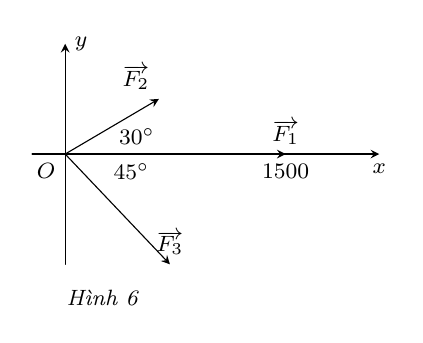
\begin{tikzpicture}[scale=0.7, font=\footnotesize, line join=round, line cap=round, >=stealth]
				\draw[->] (0.7,0)--(1.3,0) node[below left]{$O$}--(7,0) node[below]{$x$};
				\draw[->] (1.3,-2) --(1.3,2) node[right]{$y$};
				\draw[->] (1.3,0)--(5.3,0) node[above]{$\overrightarrow{F_1}$};
				\draw[](5.3,0) node[below]{$1500$};
				\draw[->] (1.3,0)--(3,1) node[above left]{$\overrightarrow{F_2}$};
				\draw[->] (1.3,0)--(3.2,-2) node[above]{$\overrightarrow{F_3}$};
				\draw[] (2.1,0) node[above right]{${30^\circ}$};
				\draw[] (2,0) node[below right]{${45^\circ}$};
				\draw[] (2,-2.3) node[below]{\textit{Hình 6}};
		\end{tikzpicture}}
		$ \overrightarrow{F_3}=(800\cos45^\circ;-800\sin45^\circ) $ hay $ \overrightarrow{F_3}=\left(400\sqrt{2};-400\sqrt{2}\right) $.\\
		Do đó, lực $ \overrightarrow{F} $ tổng hợp các lực tác động lên vật có tọa độ là\\
		$ \overrightarrow{F}=\overrightarrow{F_1}+\overrightarrow{F_2}+\overrightarrow{F_3}=\left(1500+300\sqrt{3}+400\sqrt{2};300-400\sqrt{2}\right) $.\\
		Độ lớn lực tổng hợp $ \overrightarrow{F} $ tác động lên vật là $$ |\overrightarrow{F}|=\sqrt{\left(1500+300\sqrt{3}+400\sqrt{2}\right)^2+\left(300-400\sqrt{2}\right)^2}\approx 2\,599 \text{ (N)}. $$
	}
\end{vd}
\begin{vd}[SBT KNTT]%[0H9H2-7]
	Trên màn hình ra đa của đài kiểm soát không lưu (được coi như mặt phẳng tọa độ $ Oxy $ với đơn vị trên các trục tính theo ki-lô-mét), một máy bay trực thăng chuyển động thẳng đều từ thành phố $ A $ có tọa độ $ (600;200) $ đến thành phố $ B $ có tọa độ $ (200;500) $ và thời gian bay quãng đường $ AB $ là $ 3 $ giờ. Hãy tìm tọa độ của máy bay trực thăng tại thời điểm sau khi xuất phát $ 1 $ giờ.
	\loigiai{
		Giả sử $ M(x;y) $ là vị trí của máy bay trực thăng tại thời điểm sau xuất phát $ 1 $ giờ.\\
		Ta có $ \overrightarrow{AM}=(x-600;y-200) $, $ \overrightarrow{AB}=(-400;300) $.\\
		Vì máy bay trực thăng chuyển động thẳng đều nên $ \overrightarrow{AM}=\dfrac{1}{3}\overrightarrow{AB} $. Do đó 
		$$ \heva{&x-600=-\dfrac{400}{3}\\&y-200=100} \Leftrightarrow \heva{&x=\dfrac{1400}{3}\\&y=300.} $$
		Vậy vị trí của máy bay trực thăng tại thời điểm sau khi xuất phát $ 1 $ giờ là $ M\left( \dfrac{1400}{3};300\right) $.
	}
\end{vd}

%-----------------------------------------------------------------------------
\subsection{Bài tập rèn luyện}
\ind{PHẦN I.} \inden{Câu trắc nghiệm nhiều phương án lựa chọn. Mỗi câu hỏi học sinh chỉ chọn một phương án.}\\
\setcounter{ex}{0}
\Opensolutionfile{ans}[ans/0H1-Bai1-TN]% 20câu

\begin{ex}[Trích đề kiểm tra Toán 10 GHKII THPT Phan Bội Châu- Bình Thuận NH24-25]%[0H9N1-1]
    Trong mặt phẳng $ Oxy$, cho vectơ $\overrightarrow{a}=3\overrightarrow{j}-\overrightarrow{i}$. Tọa độ của $\overrightarrow{a}$ là
    \choice
    {\True $\left(-1;3\right)$}
    {$\left(3;-1\right)$}
    {$\left(1;-3\right)$}
    {$\left(-3;1\right)$}
    \loigiai{
        Ta có $\overrightarrow{a}=3\overrightarrow{j}-\overrightarrow{i}\Leftrightarrow \overrightarrow{a}=(-1;3)$.
    }
\end{ex}
\begin{ex}[Trích đề giữa kì 2- THPT Thanh Miện, Tỉnh Hải Dương Năm học 2024 2025]%[0H9N1-1]
	Trong mặt phẳng tọa độ $Oxy$, cho $A(-3;2)$, $B(5;-4)$. Tọa độ trung điểm $AB$ là
	\choice
	{\True$(1;-1)$}
	{$(8;-6)$}
	{$(-1;1)$}
	{$(4;-3)$}
	\loigiai{
		Tọa độ trung điểm $AB$ là $\left(\dfrac{-3+5}{2};\dfrac{2+(-4)}{2}\right)=(1;-1)$.
	}
\end{ex}
\begin{ex}[Trích đề kiểm tra Toán 12 HKII Sở Bắc Ninh NH24-25]%[0H9N1-1]
	Trong mặt phẳng tọa độ $Oxy$, cho vectơ $\overrightarrow{AB} = (3;1)$ và điểm $A(-2;5)$. Tọa độ điểm $B$ là
	\choice
	{\True $(1; 6)$}
	{$(-5; 4)$}
	{$(5; -4)$}
	{$(-6; 5)$}
	\loigiai{
		Gọi $B(x_B; y_B)$. \\Ta có $\overrightarrow{AB} = (x_B - x_A; y_B - y_A) = (x_B + 2; y_B - 5)$. \\
		Vì $\overrightarrow{AB} = (3;1)$ nên $\heva{&x_B + 2 = 3\\&y_B - 5 = 1}  \Leftrightarrow \heva{&x_B=1\\&y_B =6.}$ \\
		Vậy $B(1;6)$.
	}
\end{ex}
\begin{ex}[Trích đề kiểm tra Toán khối 10 GHKII THPT C Hải Hậu - Nam Định NH24-25]%[0H9N1-2]
	Trong mặt phẳng $Oxy$, cho $\overrightarrow{a}=(1; 3)$, $\overrightarrow{b}=(2; 6)$. Khi đó $(-\overrightarrow{a}+\overrightarrow{b}) \cdot \overrightarrow{b}$ bằng
	\choice
	{\True $ 20 $}
	{$ -20 $}
	{$ -16 $}
	{$ 16 $}
\loigiai{
	Ta có $ -\overrightarrow{a}+\overrightarrow{b}=(1;3) $.\\
	Suy ra $(-\overrightarrow{a}+\overrightarrow{b}) \cdot \overrightarrow{b}=1\cdot 2+3\cdot 6=20$.
}
\end{ex}
\begin{ex}[Trích đề kiểm tra giữa kì 2- THPT Thanh Miện, Tỉnh Hải Dương-Năm học 2024 2025]%[0H9N1-2]
	Trong mặt phẳng tọa độ $Oxy$, cho $\overrightarrow{a}=(1;2)$, $\overrightarrow{b}=(3;-3)$. Tọa độ của vectơ $\overrightarrow{c}=3\overrightarrow{a}-2\overrightarrow{b}$ là
	\choice
	{$(9;0)$}
	{$(3;12)$}
	{$(-3;0)$}
	{\True$(-3;12)$}
	\loigiai{
		Ta có $\overrightarrow{c}=3\overrightarrow{a}-2\overrightarrow{b}=(3\cdot1-2\cdot3;3\cdot2-2\cdot(-3))=(-3;12)$.
	}
\end{ex}
\begin{ex}[Trích đề kiểm tra Toán 12 HKII THPT Nguyễn An Ninh - HCM NH24-25]%[0H9N1-2]
	Trong mặt phẳng $\mathrm{Oxy}$, cho $A(9;-11)$, $B(-3;13)$. Tọa độ trung điểm $I$ của đoạn thẳng $AB$ là
	\choice
	{\True $I(3;1)$}
	{$I(6;-12)$}
	{$I(-6;12)$}
	{$I(-12;-2)$}
	\loigiai{
		Gọi $I(x_I; y_I)$ là trung điểm của đoạn thẳng $AB$.\\
		Khi đó $\heva{x_I = \dfrac{x_A+x_B}{2} = \dfrac{9+(-3)}{2}=3 \\ y_I = \dfrac{y_A+y_B}{2} = \dfrac{-11+13}{2}=1.}$\\
		Vậy tọa độ trung điểm là $I(3;1)$.
	}
\end{ex}
\begin{ex}[Trích đề kiểm tra Toán khối 10 GHKII THPT C Hải Hậu - Nam Định NH24-25]%[0H9N1-3]
	Trong mặt phẳng $Oxy$, cho điểm các điểm $A(0; 3)$, $B(4; 0)$, $C(-4;-3)$. Tọa độ trọng tâm của tam giác $\triangle ABC$ là
	\choice
	{$(0; 1)$}
	{$(-1; 0)$}
	{$(1; 0)$}
	{\True $(0; 0)$}
\loigiai{
	Gọi $ G $ là trọng tâm của $ \triangle ABC $, khi đó
	$$ \heva{& x_G=\dfrac{x_A+x_B+x_C}{3}=\dfrac{0+4+(-4)}{3}=0 \\ & y_G=\dfrac{y_A+y_B+y_C}{3}=\dfrac{3+0+(-3)}{3}=0.} $$
	Vậy $ G(0;0) $.
}
\end{ex}
\begin{ex}[Trích đề kiểm tra Toán 10 GHKII THPT Chuyên Lê Quý Đôn Ninh Thuận NH24-25]%[0H9N1-3]
	Trong hệ trục tọa độ $(O,i,j)$, cho $\overrightarrow{OM}=\overrightarrow{i}-3\overrightarrow{j}$. Khẳng định nào sau đây \textbf{đúng}?
	\choice
	{$M(-1;3)$}
	{$M(0;-3)$}
	{\True $M(1;-3)$}
	{$M(3;-1)$}
	\loigiai{
		Tọa độ của điểm $M$ là tọa độ của vectơ $\overrightarrow{OM}=\overrightarrow{i}-3\overrightarrow{j}$.\\
		Vậy tọa độ của điểm $M$ là $(1; -3)$.
	}
\end{ex}
\begin{ex}[Trích đề toán 10 - GHKII - THPT Chuyên Lương Thế Vinh - Tỉnh Đồng Nai - NH 24-25]%[0H9N1-3]
	Trong mặt phẳng tọa độ $Oxy$ cho $A(1; -1)$, $B(3; 4)$. Trung điểm $M$ của $AB$ có tọa độ là
	\choice
	{ $(2; 5)$ }
	{ $\left( 1; \dfrac{5}{2} \right)$ }
	{ $(4; 3)$ }
	{\True $\left( 2; \dfrac{3}{2} \right)$ }
	\loigiai{
		Vì $M$ là trung điểm của $AB$ nên $M$ tọa độ là $\left(2; \dfrac{3}{2}\right)$.
	}
\end{ex}
\begin{ex}[Trích đề kiểm tra Toán 10 HKI THPT Chuyên Trần Phú - Hải Phòng NH24-25]%[0H9N1-3]
	Trong mặt phẳng tọa độ $O x y$, cho $\overrightarrow{a}=4 \overrightarrow{j}-\overrightarrow{i}$. Tọa độ của vectơ $\overrightarrow{a}$ là
	\choice
	{$\overrightarrow{a}=(4 ;-1)$}
	{$\overrightarrow{a}=(-1 ;-4)$}
	{\True $\overrightarrow{a}=(-1 ; 4)$}
	{$\overrightarrow{a}=(-4 ; 1)$}
	\loigiai{
		Do $\overrightarrow{a}=4 \overrightarrow{j}-\overrightarrow{i}$ nên tọa độ của $\overrightarrow{a}=(-1;4)$.
	}
\end{ex}
\begin{ex}[Trích đề kiểm tra toán 10 HK2 THPT Marie Curie - Hồ Chí Minh - Năm học 2024-2025]%[0H9N1-3]
	Trong mặt phẳng toạ độ $Oxy$, cho hai điểm $A(-3;-1)$ và $B(1; 1)$. Toạ độ trung điểm $M$ của đoạn thẳng $AB$ là
	\choice
	{$M(4; 2)$}
	{$M(2;1)$}
	{$M(-2; -1)$}
	{\True $(-1;0)$}
	\loigiai{Trung điểm $M$ của đoạn thẳng $AB$ có tọa độ $M\left(\dfrac{-3+1}{2};\dfrac{-1+1}{2} \right) $ hay $M(1;0)$.}
\end{ex}
\begin{ex}[Trích đề kiểm tra Khối 10 HK2 THPT CHUYÊN LÊ QUÝ ĐÔN - NINH THUẬN NH24-25]%[0H9N1-3]
	Trong mặt phẳng tọa độ $Oxy$, cho $A(-2;1)$, $\overrightarrow{v}= (3;-2)$. Điểm $B$ thỏa $\overrightarrow{AB} = \overrightarrow{v}$ là
	\choice
	{$B(1;-1)$}
	{\True $B(-1;1)$}
	{$B(5;-3)$}
	{$B(-5;3)$}
	\loigiai{
		Gọi tọa độ điểm $B$ là $(x_B; y_B)$.\\
		Ta có $\overrightarrow{AB} = \overrightarrow{v}$, suy ra
		$\heva{&x_B + 2 = 3 \\&y_B - 1 = -2}$ hay $\Leftrightarrow \heva{&x_B = 1 \\&y_B = -1.}$\\
		Vậy điểm $B$ có tọa độ $(1;-1)$.
	}
\end{ex}
\begin{ex}[Trích đề kiểm tra Toán 10 GHKII THPT Chuyên Lê Quý Đôn - Ninh Thuận NH24-25]%[0H9N2-1]
	Trong hệ trục tọa độ $Oxy$, cho hai điểm $\overrightarrow{a}=(1;1)$, $\overrightarrow{b}=(4;-1)$. Tính tích vô hướng của hai vectơ $\overrightarrow{a}$, $\overrightarrow{b}$ bằng
	\choice
	{$\sqrt{13}$}
	{$5$}
	{\True $3$}
	{$(3;-2)$}
	\loigiai{
		Tích vô hướng của hai vectơ $\overrightarrow{a}$ và $\overrightarrow{b}$ là
		$\overrightarrow{a}\cdot\overrightarrow{b}=1\cdot4+1\cdot(-1)=4-1=3$.
	}
\end{ex}
\begin{ex}[Trích đề kiểm tra Toán 10 HKI THPT TX Quảng Trị NH24-25]%[0H9H2-1]
	Trong hệ tọa độ $Oxy$, cho $\overrightarrow{u}=3\overrightarrow{j}-\overrightarrow{i}$; $\overrightarrow{v}=(2;-1)$. Tính biểu thức tọa độ của $\overrightarrow{u}\cdot\overrightarrow{v}$.
	\choice
	{$\overrightarrow{u}\cdot\overrightarrow{v}=7$}
	{\True $\overrightarrow{u}\cdot\overrightarrow{v}=(2;-3)$}
	{$\overrightarrow{u}\cdot\overrightarrow{v}=5\sqrt{2}$}
	{$\overrightarrow{u}\cdot\overrightarrow{v}=-5 $}
	\loigiai{
		Ta có $\overrightarrow{u}=(-1; 3)$, $\overrightarrow{v}=(2;-1)$\\
		Tích vô hướng giữa hai vectơ là
		$\overrightarrow{u}\cdot\overrightarrow{v}=(-1)\cdot(2)+(3)\cdot(-1)=-2- 3=-5$.
	}
\end{ex}
\begin{ex}%[0H9H1-4]
	Trong mặt phẳng tọa độ, cặp vec-tơ nào sau đây có cùng phương
	\choice
	{$\overrightarrow{u}=(2;3)$ và $\overrightarrow{v}=\left(\dfrac{1}{2};6\right)$}
	{\True $\overrightarrow{a}=(\sqrt{2};6)$ và $\overrightarrow{b}=(1;3\sqrt{2})$}
	{$\overrightarrow{i}=(0;1)$ và $\overrightarrow{j}=(1;0)$}
	{$\overrightarrow{c}=(1;3)$ và $\overrightarrow{d}=(2;-6)$}
	\loigiai{
		Cặp vec-tơ $\overrightarrow{a}=\left(\sqrt{2};6\right)$ và $\overrightarrow{b}=\left(1;3\sqrt{2}\right)$ cùng phương vì $\overrightarrow{a}=\sqrt{2}\overrightarrow{b}$.
	}
\end{ex}
\begin{ex}%[0H9H2-4]
	Trong mặt phẳng tọa độ, cặp vectơ nào sau đây vuông góc với nhau?
	\choice
	{$\overrightarrow{u}=(2;3)$ và $\overrightarrow{v}=(4;6)$}
	{$\overrightarrow{a}=(1;-1)$ và $\overrightarrow{b}=(-1;1)$}
	{\True $\overrightarrow{z}=(a;b)$ và $\overrightarrow{t}=(-b;a)$}
	{$\overrightarrow{n}=(1;1)$ và $\overrightarrow{k}=(2;0)$}
	\loigiai{
		Cặp vec-tơ $\overrightarrow{z}=(a;b)$ và $\overrightarrow{t}=(-b;a)$ vuông góc với nhau vì $\overrightarrow{z}\cdot \overrightarrow{t}=a\cdot (-b)+b\cdot a=0$.
	}
\end{ex}
\begin{ex}%[0H9H2-3]
	Trong mặt phẳng tọa độ, vectơ nào sau đây có độ dài bằng $1$?
	\choice
	{$\overrightarrow{a}=(1;1)$}
	{$\overrightarrow{b}=(1;-1)$}
	{$\overrightarrow{c}=\left(2;\dfrac{1}{2}\right)$}
	{\True $\overrightarrow{d}=\left(\dfrac{1}{\sqrt{2}};-\dfrac{1}{\sqrt{2}}\right)$}
	\loigiai{
		Vec-tơ có độ dài bằng $1$ là vec-tơ $\overrightarrow{d}=\left(\dfrac{1}{\sqrt{2}};-\dfrac{1}{\sqrt{2}}\right)$.\\
		Có: $|\overrightarrow{d}|=\sqrt{\left(\dfrac{1}{\sqrt{2}}\right)^2+\left(-\dfrac{1}{\sqrt{2}}\right)^2}=1$.
	}
\end{ex}
\begin{ex}%[0H9H2-2]
	Góc giữa vectơ $\overrightarrow{a}=(1;-1)$ và vectơ $\overrightarrow{b}=(-2;0)$ có số đo bằng
	\choice
	{$90^\circ$}
	{$0^\circ$}
	{\True $135^\circ$}
	{$45^\circ$}
	\loigiai{
		Có: $\cos (\overrightarrow{a};\overrightarrow{b})=\dfrac{\overrightarrow{a}\cdot \overrightarrow{b}}{|\overrightarrow{a}|\cdot |\overrightarrow{b}|}=\dfrac{1\cdot (-2)+(-1)\cdot 0}{\sqrt{1^2+(-1)^2}\cdot \sqrt{(-2)^2+0^2}}=-\dfrac{1}{\sqrt{2}}$.\\
		Vậy góc giữa hai $\overrightarrow{a}$ và $\overrightarrow{b}$ bằng $135^\circ$.
	}
\end{ex}
\begin{ex}[SBT KNTT]%[0H9H2-2]
	Cosin góc giữa hai vectơ $ \overrightarrow{u}=(1;1) $ và $ \overrightarrow{v}=(-2;1) $ là 
	\choice
	{$-\dfrac{1}{10}$}
	{$\dfrac{\sqrt{10}}{10}$}
	{\True $-\dfrac{\sqrt{10}}{10}$}
	{$\dfrac{3}{10}$}
	\loigiai{
		Ta có $\cos \left(\overrightarrow{u},\overrightarrow{v}\right)=\dfrac{1\cdot (-2)+1\cdot 1}{\sqrt{1^2+1^2}\cdot\sqrt{(-2)^2+1^2}}=-\dfrac{\sqrt{10}}{10}$.
	}
\end{ex}

\begin{ex}[SBT KNTT]%[0H9H2-4]
	Cho tam giác $ ABC $ có $ A(2;6) $, $ B(-2;2) $, $ C(8;0) $. Khi đó, tam giác $ ABC $ là
	\choice
	{tam giác đều}
	{\True tam giác vuông tại $ A $}
	{tam giác có góc tù tại $ A $}
	{tam giác cân tại $ A $}
	\loigiai{ Ta có $ \overrightarrow{AB}=(-4;-4) $, $ \overrightarrow{AC}=(6;-6) $.\\
		Vì $ \overrightarrow{AB}\cdot \overrightarrow{AC}=(-4)\cdot 6+(-4)\cdot (-6)=0 $ nên tam giác $ ABC $ vuông tại $ A $.
	}
\end{ex}
\Closesolutionfile{ans}

\ind{PHẦN II.} \inden{Câu trắc nghiệm đúng sai. Trong mỗi ý a), b), c), d) ở mỗi câu, học sinh chọn đúng hoặc sai.}\\
\setcounter{ex}{0}
\Opensolutionfile{ans}[ans/0H1-Bai1-DS]% 5câu
\begin{ex}%[0H9H1-5]
	Trong mặt phẳng tọa độ $Oxy$, cho các vectơ $\overrightarrow{a}=(2;-2)$, $\overrightarrow{b}=(4; 1)$ và $\overrightarrow{c}=(0;-1)$. Khi đó
	\choiceTF
	{\True $2\overrightarrow{a}-\overrightarrow{b}-3\overrightarrow{c}=(0;-2)$}
	{\True Vectơ $\overrightarrow{e}=(1;-1)$ cùng phương, cùng hướng với vectơ $\overrightarrow{a}$}
	{Vectơ $\overrightarrow{f}=\left(-1;-\dfrac{1}{4}\right)$ cùng phương, cùng hướng với vectơ $\overrightarrow{b}$}
	{\True $\overrightarrow{a}=\dfrac{1}{2} \overrightarrow{b}+\dfrac{5}{2} \overrightarrow{c}$}
	\loigiai{
		\begin{itemchoice}
			\itemch Đúng. Ta có $\heva{&2 \overrightarrow{a}=(4;-4) \\&-\overrightarrow{b}=(-4;-1) \\&-3 \overrightarrow{c}=(0; 3)} \Rightarrow \overrightarrow{d}=2 \overrightarrow{a}-\overrightarrow{b}-3 \overrightarrow{c}=(0;-2)$.
			\itemch Đúng.  Ta $\overrightarrow{a}=(2;-2)=2 \overrightarrow{e}$ nên $\overrightarrow{a}$, $\overrightarrow{e}$ là hai vectơ cùng phương với nhau, hơn nữa chúng cùng hướng với nhau vì $\overrightarrow{a}=k \overrightarrow{e}$, $k=2>0$.
			\itemch Sai. Tương tự: $\overrightarrow{b}=(4; 1)=-4 \overrightarrow{f}$, tức là $\overrightarrow{b}=k \overrightarrow{f}$, $k=-4<0$ nên $\overrightarrow{b}$ và $\overrightarrow{f}$ là hai vectơ cùng phương, ngược hướng với nhau.
			\itemch Đúng. Gọi $m$, $n$ là các số thỏa mãn $\overrightarrow{a}=m \overrightarrow{b}+n \overrightarrow{c}$ ($\overrightarrow{b}$, $\overrightarrow{c}$ không cùng phương).\\
			Khi đó $\heva{&2=m \cdot 4+n \cdot 0 \\&-2=m \cdot 1+n \cdot(-1)} \Leftrightarrow\heva{&m=\dfrac{1}{2} \\&n=\dfrac{5}{2}}$. Vậy $\overrightarrow{a}=\dfrac{1}{2} \overrightarrow{b}+\dfrac{5}{2} \overrightarrow{c}$.
		\end{itemchoice}
	}
\end{ex}
\begin{ex}[Trích đề kiểm tra THPT Thị Xã Quảng Trị  - Quảng Trị NH24-25]%[0H9H2-5]
	Trong mặt phẳng tọa độ $Oxy$, cho tam giác $ABC$ có $A(-3;0)$, $B(3;0)$ và $C(3;6)$. 
	\choiceTF
	{\True $\overrightarrow{AC}=(6;6)$}
	{$\overrightarrow{AB}\cdot \overrightarrow{BC}=8$}
	{$\overrightarrow{AB}$ vuông góc với trục $Ox$}
	{Điểm $H(1;5)$ là trực tâm của tam giác $ABC$}
	\loigiai{
		\begin{itemchoice}
			\itemch $\overrightarrow{AC}=(3-(-3);6-0)=(6;6)$.
			\itemch Ta có $\overrightarrow{AB}=(6;0)$ và $\overrightarrow{BC}=(0;6)$.\\
			Suy ra $\overrightarrow{AB}\cdot \overrightarrow{BC}=6\cdot 0+0\cdot 6=0$.
			\itemch Xét $\overrightarrow{i}=(1;0)$.\\
			Ta có $\overrightarrow{AB}\cdot \overrightarrow{i}=6\cdot 1+0\cdot 0=6$.\\
			Suy ra $\overrightarrow{AB}$ không vuông góc với $\overrightarrow{i}$.\\
			Vậy $\overrightarrow{AB}$ không vuông góc với trục $Ox$.
			\itemch Gọi $H(x;y)$ là trực tâm của tam giác $ABC$.\\
			Suy ra $\overrightarrow{AH}=(x+3;y)$ và $\overrightarrow{CH}=(x-3;y-6)$.\\
			Ta có 
			\begin{eqnarray*}
				& &\heva{&\overrightarrow{AH}\perp \overrightarrow{BC}\\&\overrightarrow{CH}\perp AB}\\
				&\Leftrightarrow& \heva{&\overrightarrow{AH}\cdot \overrightarrow{BC}=0\\&\overrightarrow{CH}\cdot \overrightarrow{AB}=0}\\
				&\Leftrightarrow& \heva{&(x+3)\cdot 0+y\cdot6=0\\&(x-3)\cdot 6+(y-6)\cdot 0=0}\\
				&\Leftrightarrow& \heva{&y=0\\&x=3.}
			\end{eqnarray*}
			Vậy $H(0;3)$.
		\end{itemchoice}
	}
\end{ex}
\begin{ex}[Trích đề kiểm tra Toán 10 GHKII THPT Nguyễn Chí Thanh NH24-25]%[0H9H2-1]
	Cho $\overrightarrow{AB}=(-3 ; 2)$ và $A(1 ;-2)$, $\overrightarrow{a}=-2 \overrightarrow{j}+3 \overrightarrow{i}$. Khi đó
	\choiceTF
	{\True Tọa độ của $-2 \overrightarrow{a}=(-6 ; 4)$}
	{\True Tọa độ của điểm $B(-2 ; 0)$}
	{Tọa độ của $\overrightarrow{a}=(-2 ; 3)$}
	{Tích vô hướng $\overrightarrow{AB} \cdot \overrightarrow{a}$ là $ 10 $}
	\loigiai{
		\begin{itemchoice}
			\itemch \textbf{Đúng}.\\
			Ta có $ \overrightarrow{a}=(3;-2) $ nên $ -2\overrightarrow{a}=(-2\cdot 3; -2 \cdot (-2))=(-6;4) $.
			\itemch \textbf{Đúng}.\\
			Ta có $ \overrightarrow{AB}=(-3;2)\Leftrightarrow \heva{&x_B-1=-3\\&y_B-(-2)=2}\Leftrightarrow \heva{&x_B=-2\\&y_B=0.}$\\
			Nên $ B(-2;0) $.
			\itemch \textbf{Sai}.\\
			Ta có $ \overrightarrow{a}=(3;-2) $.
			\itemch \textbf{Sai}.\\
			Ta có $\overrightarrow{AB} \cdot \overrightarrow{a}=-3\cdot 3 + 2 \cdot (-2)=-13$.
		\end{itemchoice}
	}
\end{ex}
\begin{ex}[Trích đề kiểm tra Toán 10 HKI THPT Chuyên Trần Phú - Hải Phòng NH24-25]%[0H9H2-2]
Trong mặt phẳng với hệ tọa độ $O x y$, cho $\triangle A B C$ với $A(-2 ; 5)$, $B(-4 ;-2)$, $C(1 ; 5)$. Các khẳng định sau đây là \textbf{đúng} hay \textbf{sai}?
\choiceTF
{Toạ độ vectơ $\overrightarrow{u}=2 \overrightarrow{AB}+\overrightarrow{AC}$ là $(1 ; 14)$}
{Trọng tâm $G$ của tam giác có tọa độ là $\left(-\dfrac{5}{3} ;-\dfrac{8}{3}\right)$}
{\True Độ dài $A B=\sqrt{53}$}
{\True $\cos \left(\overrightarrow{AB}, \overrightarrow{CG}\right)>0{,}8$ với $G$ là trọng tâm của tam giác $ABC$}
\loigiai{
	Ta có $ \overrightarrow{AB}=(-2;-7) $ và $ \overrightarrow{AC}=(3;0) $.\\
	Do $ G $ là trọng tâm của $ \triangle ABC $ nên $ \heva{&x_G=\dfrac{-2+(-4)+1}{3}=-\dfrac{5}{3}\\&y_G=\dfrac{5+(-2)+5}{3}=\dfrac{8}{3}} $ dẫn đến  $ G\left(-\dfrac{5}{3} ;\dfrac{8}{3}\right) $.
\begin{itemchoice}
\itemch Tọa độ của vectơ $\overrightarrow{u}=2 \overrightarrow{AB}+\overrightarrow{AC}=\left(2\cdot (-2)+3;2\cdot (-7)+0\right)=(-1;-14)$.
\itemch Ta đã có $ G\left(-\dfrac{5}{3} ;\dfrac{8}{3}\right) $.
\itemch Ta có độ dài $ AB=\sqrt{(-2)^2+7^2}=\sqrt{53} $.
\itemch Ta có $ \overrightarrow{CG}=\left(-\dfrac{8}{3};-\dfrac{7}{3}\right) $.\\
Khi đó $\cos (\overrightarrow{AB}, \overrightarrow{C G})=\dfrac{\left|(-2)\cdot \left(-\dfrac{8}{3}\right)+(-7)\cdot \left(-\dfrac{7}{3}\right)\right|}{\sqrt{(-2)^2+(-7)^2}\cdot \sqrt{\left(-\dfrac{8}{3}\right)^2+\left(-\dfrac{7}{3}\right)^2}}\approx 0{,}83>0{,}8$.
\end{itemchoice}
}
\end{ex}
\begin{ex}[Trích đề giữa kì 2 - THPT Thanh Miện, Tỉnh Hải Dương Năm học 2024 2025]%[0H9H2-3]
	Cho ba điểm $A(-1;1)$, $B(2;1)$, $C(-1;-3)$. Các mệnh đề sau đúng hay sai?
	\choiceTF
	{\True Điểm $N$ thuộc trục $Oy$ sao cho $N$ cách đều $B$, $C$ có tung độ bằng $-\dfrac{5}{8}$}
	{\True $\triangle ABC$ là tam giác vuông}
	{Tứ giác $ABCD$ là hình bình hành khi $D(2;-3)$}
	{\True $A$, $B$, $C$ là ba đỉnh của một tam giác}
	\loigiai{
		\begin{itemchoice}
			\itemch Gọi $N(0;y)\in Oy$, khi đó $\overrightarrow{BN}=(-2;y-1)$, $\overrightarrow{CN}=(1;y+3)$.\\
			Theo đề ta có\\
			$BN=CN\Leftrightarrow BN^2=CN^2\Leftrightarrow 4+(y-1)^2=1+(y+3)^2\Leftrightarrow y=-\dfrac{5}{8}$.
			\itemch $\overrightarrow{AB}=(3;0)$, $\overrightarrow{AC}=(0;-4)$, $\overrightarrow{BC}=(-3;-4)$.\\
			Xét $\overrightarrow{AB}\cdot\overrightarrow{AC}=3\cdot0+0\cdot(-4)=0$ nên $AB\perp AC$.\\
			Vậy tam giác $ABC$ vuông tại $A$.
			\itemch Để tứ giác $ABCD$ là hình bình hành thì $\overrightarrow{AB}=\overrightarrow{DC}\Leftrightarrow \heva{&3=-1-x_D\\& 0=-3-y_D}\Leftrightarrow \heva{&x_D=-4\\& y_D=-3.}$\\
			Vậy $D(-4;-3)$.
			\itemch Xét $\dfrac{0}{-3}\neq \dfrac{-4}{-4}$ nên $\overrightarrow{AC}$ và $\overrightarrow{BC}$ không cùng phương.\\
			Vậy $A$, $B$, $C$ có thể lập thành một tam giác.    
		\end{itemchoice}
	}
\end{ex}
\Closesolutionfile{ans}

\ind{PHẦN III.} \inden{Câu trắc nghiệm trả lời ngắn. Trong mỗi ý a), b), c), d) ở mỗi câu, học sinh chọn đúng hoặc sai.}\\
\setcounter{ex}{0}
\Opensolutionfile{ans}[ans/0H1-Bai1-TLN]% 5 câu
\begin{ex}[Trích đề thi GK2 lớp 10 THPT Nguyễn Chí Thanh-Tây Ninh năm học 2024-2025]%[0H9N1-3]
Trong mặt phẳng tọa độ $Oxy$ cho điểm $A(3;-4)$. Điểm $A'$ là hình chiếu vuông góc của điểm $A$ lên trục $Ox$. Tìm tung độ của điểm $A'$.\shortans[oly]{0}
\loigiai{
Hình chiếu vuông góc của điểm $A(x_0; y_0)$ lên trục $Ox$ là điểm $A'(x_0; 0)$.\\
Do đó, hình chiếu vuông góc của $A(3; -4)$ lên trục $Ox$ là $A'(3; 0)$.\\
Tung độ của điểm $A'$ là $0$.
}
\end{ex}
\begin{ex}[Trích đề kiểm tra Toán 10 GHKII THPT Phan Bội Châu- Bình Thuận NH24-25]%[0H9H1-3]
    Trong mặt phẳng $ Oxy$, cho hình bình hành $ADBC$ có $A\left(-3;5\right)$, $B\left(1;1\right)$, $C\left(2;3\right)$, $D\left(m;n\right)$. Giá trị của $ m+n$ bằng bao nhiêu? \shortans[oly]{-1}
    \loigiai{
        Ta có $\overrightarrow{AD}=\left(m+3;n-5\right)$, $\overrightarrow{CB}=\left(-1;-2\right)$.\\
        $ADBC$ là hình bình hành $\Leftrightarrow\overrightarrow{AD}=\overrightarrow{CB}\Leftrightarrow\left\{\begin{aligned}
            & m+3=-1\\ 
            & n-5=-2\\ 
        \end{aligned}\right.\Leftrightarrow\left\{\begin{aligned}
            & m=-4\\ 
            & n=3.\\ 
        \end{aligned}\right.$\\
        Vậy $ m+n=-1$.}
\end{ex}
\begin{ex}[Trích đề kiểm tra Toán 10 GHKII THPT Chuyên Lương Thế Vinh-Đồng Nai NH24-25]%[0H9H1-3]
	Trong mặt phẳng tọa độ $Oxy$, cho ba điểm $A(-1;-1)$, $B(0; 1)$, $C(3; 0)$ và $D(a; b)$ là điểm sao cho $ABCD$ là hình bình hành. Khi đó, độ dài $OD$ bằng bao nhiêu? (làm tròn đến hàng phần chục)
	\shortans[oly]{2,8}
	\loigiai{
	Ta có $\overrightarrow{AB}=(1;2)$ và $\overrightarrow{BC}=(3;-1)$ khi đó $\overrightarrow{AB}$ không cùng phương với $\overrightarrow{BC}$ nên tứ giác $ABCD$ là hình bình hành khi 
	$$\overrightarrow{AB}=\overrightarrow{DC}\Rightarrow \heva{&3-x=1\\&-y=2}\Rightarrow \heva{&x=2\\&y=-2.}$$
	Khi đó $D(2;-2)$.\\
	Vậy $OD=2\sqrt{2}\approx 2{,}8$.
	}
\end{ex}
\begin{ex}[Trích đề kiểm tra Toán 10 HKI THPT Chuyên Lê Quý Đôn Năm học 24-25]%[0H9H2-7]
	Một chiếc phà chở khác qua sông từ điểm $A(30;2)$ đến điểm $B(-60;2)$ đối diện bên kia sông ($AB$ vuông góc với bờ sông). Nhưng vì có gió và nước chảy mạnh nên chiếc phà chạy theo phương lệch so với phương vuông góc với bờ sông một góc $30^\circ$. Hỏi vị trí của điểm đến của phà bên bờ bên kia cách $B$ bao nhiêu? (làm tròn kết quả đến hàng phần chục).
	\shortans[oly]{52,0}
	\loigiai{
		\immini{Ta có $AB=\sqrt{(-60-30)^2+(2-2)^2}=90$.\\
			Suy ra $BC=AB\cdot \tan 30^\circ=30\sqrt{3}\approx 52{,}0$.}{\begin{tikzpicture}[scale=1, font=\footnotesize, line join=round, line cap=round, >=stealth]
				\path 
				(0,0) coordinate (A)
				+(90:2) coordinate (B)
				(B)+(180:1.5) coordinate (C)
				;
				\foreach \x/\dinh/\y in {A/B/C} \draw[fill = gray!50] ($(\dinh)!3pt!(\x)$)--($(\dinh)!3pt!(\x)+(\dinh)!3pt!(\y)-(\dinh)$)--($(\dinh)!3pt!(\y)$)--(\dinh)--cycle; 
				\draw    pic["$30^\circ$", draw=black, angle eccentricity=1.2, angle radius=0.8cm]
				{angle=B--A--C}; %góc
				\draw (A)--(B)--(C)--cycle;
				\foreach \p/\r in {A/-90,B/90,C/90}
				\fill (\p) circle (1.5pt) node[shift={(\r:3mm)}]{$\p$};
		\end{tikzpicture}}
	}
\end{ex}

\begin{ex}%[0H9V1-6]
	\immini{Trên màn hình ra đa của đài kiểm soát không lưu (được coi như mặt phẳng tọa độ $O x y$ với đơn vị trên các trục tính theo ki-lô-mét), một máy bay trực thăng chuyển động thẳng đều từ thành phố $A$ có tọa độ $(400 ; 50)$ đến thành phố $B$ có tọa độ $(100 ; 450)$ (Hình bên) và thời gian bay quãng đường $A B$ là $3$ giờ. Gọi $M(a; b)$ là tọa độ của máy bay trực thăng tại thời điểm sau khi xuất phát $2$ giờ, trong đó $b$ là phân số tối giản. Tính giá trị biểu thức $T=\dfrac{3}{200}\cdot a\cdot b$.}
	{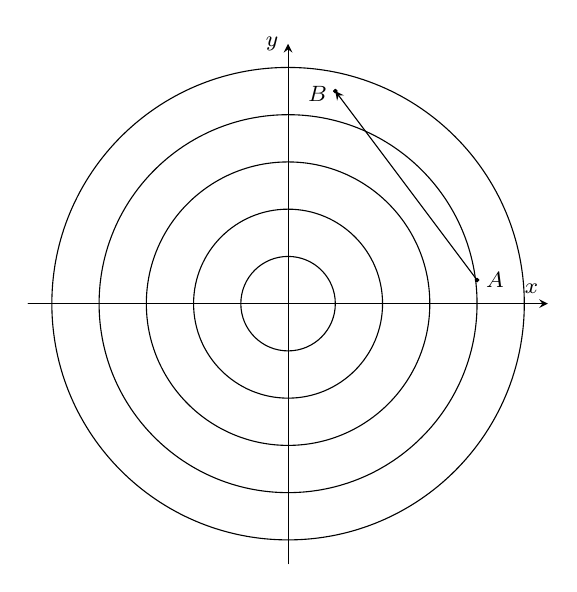
\begin{tikzpicture}[>=stealth,line join=round,line cap=round,font=\footnotesize,scale=0.6]
			\draw[->] (-5.5,0)--(0,0)--(5.5,0)node[above left]{$x$};
			\draw[->] (0,-5.5)--(0,5.5)node[left]{$y$};
			\path 
			(4,0.5) coordinate (A)
			(1,4.5) coordinate (B);
			\draw (0,0) circle (1) (0,0) circle (2)(0,0) circle (3)(0,0) circle (4)(0,0) circle (5);
			\draw[->](A)--(B);
			\foreach \x/\y in {A/0,B/190}
			\draw[fill=black] (\x) circle (1.1pt) + (\y:0.38cm) node{$\x$};
	\end{tikzpicture}}
	\shortans[oly]{950}
	\loigiai{
		Gọi $M(a; b)$ là tọa độ của máy bay trực thăng tại thời điểm sau khi xuất phát $2$ giờ.
		Ta có $\overrightarrow{A M}=(a-400 ; b-50)$ và $\overrightarrow{AB}=(-300 ; 400)$.\\
		Do máy bay chuyển động thẳng đều nên quãng đường máy bay đi được sau $2$ giờ bằng $\dfrac{2}{3}$ tổng quãng đường hay $A M=\dfrac{2}{3} A B$.\\
		Mà $M$ thuộc đoạn $A B$ nên $\overrightarrow{A M}=\dfrac{2}{3} \overrightarrow{AB}$.\\
		Suy ra $\heva{&a-400=\dfrac{2}{3} \cdot(-300) \\& b-50=\dfrac{2}{3} \cdot 400} \Leftrightarrow\heva{&a=200 \\& b=\dfrac{950}{3}.}$\\
		Vậy $M\left(200;\dfrac{950}{3}\right)$.\\
		Vậy $a=200$ và $b=\dfrac{950}{3}$ nên $T=\dfrac{3}{200}\cdot 200\cdot \dfrac{950}{3}=950$.}
\end{ex}

\Closesolutionfile{ans}

\ind{PHẦN IV.} \inden{Tự luận.}\\% 10 câu
\setcounter{ex}{0}
\begin{ex}%[0H9H1-1]
	Trong mặt phẳng tọa độ $Oxy$, cho $A(2;1)$, $B(-2;5)$ và $C(-5;2)$.
	\begin{enumerate}
		\item Tìm tọa độ của các vectơ $\overrightarrow{BA}$ và $\overrightarrow{BC}$.
		\item Chứng minh rằng $A$, $B$, $C$ là ba đỉnh của một tam giác vuông. Tính diện tích và chu vi của tam giác đó.
		\item Tìm tọa độ trọng tâm $G$ của tam giác $ABC$.
		\item  Tìm tọa độ của điểm $D$ sao cho tứ giác $BCAD$ là một hình bình hành.
	\end{enumerate}
	
	\loigiai{
		\begin{enumerate}
			\item Ta có $\overrightarrow{BA}=(4;-4)$ và $\overrightarrow{BC}=(-3;-3)$.
			\item 
			\begin{itemize}
				\item Do $\overrightarrow{BA}=(4;-4)$ và $\overrightarrow{BC}=(-3;-3)$ nên $\overrightarrow{BA}$ và $\overrightarrow{BC}$ không cùng phương hay $A$, $B$, $C$ là ba đỉnh của một tam giác.\\
				Mặt khác $\overrightarrow{BA}\cdot \overrightarrow{BC}=4\cdot(-3)-4\cdot(-3)=0$ nên tam giác $ABC$ vuông tại $B$.
				\item $BA=\sqrt{16+16}=4\sqrt{2}$, $BC=\sqrt{9+9}=3\sqrt{2}$, $AC=\sqrt{49+1}=5\sqrt{2}$.\\
				Diện tích của tam giác $ABC$ là $S_{ABC}=\dfrac{1}{2}\cdot BA\cdot BC=\dfrac{1}{2}\cdot 4\sqrt{2}\cdot 3\sqrt{2}=12$.\\
				Chu vi của tam giác $ABC$ là $2P=AB+AC+BC=4\sqrt{2}+5\sqrt{2}+3\sqrt{2}=12\sqrt{2}$.
			\end{itemize}
			\item Tọa độ trọng tâm $G$ của tam giác $ABC$ là $\heva{&x_G=\dfrac{x_A+x_B+x_C}{3}=-\dfrac{5}{3}\\&y_G=\dfrac{y_A+y_B+y_C}{3}=\dfrac{8}{3}} \Rightarrow G\left(-\dfrac{5}{3};\dfrac{8}{3}\right)$.
			\item Tứ giác $BCAD$ là một hình bình hành\\ $ \Leftrightarrow \overrightarrow{BC}=\overrightarrow{DA} \Leftrightarrow \heva{&x_A-x_D=-3\\&y_A-y_D=-3} \Leftrightarrow \heva{&x_D=5\\&y_D=4.}$\\
			Vậy $D=\left(5;4\right)$.
		\end{enumerate}
	}
\end{ex}

\begin{ex}%[0H9H1-1]
	Trong mặt phẳng tọa độ $Oxy$, cho $A(1;2)$, $B(3;4)$, $C(-1;-2)$ và $D(6;5)$.
	\begin{enumerate}
		\item Tìm tọa độ của các vectơ $\overrightarrow{AB}$ và $\overrightarrow{CD}$.
		\item Hãy giải thích tại sao các vectơ $\overrightarrow{AB}$ và $\overrightarrow{CD}$ cùng phương.
		\item Giả sử $E$ là điểm có tọa độ $(a;1)$. Tìm $a$ để các vectơ $\overrightarrow{AC}$ và $\overrightarrow{BE}$ cùng phương.
		\item  Với $a$ tìm được, hãy biểu thị vectơ $\overrightarrow{AE}$ theo các vectơ $\overrightarrow{AB}$ và $\overrightarrow{AC}$.
	\end{enumerate}
	\loigiai{
		\begin{enumerate}
			\item $\overrightarrow{AB}=\left(2;2\right)$ và $\overrightarrow{CD}=\left(7;7\right)$.
			\item Do $\dfrac{2}{7}=\dfrac{2}{7}$ nên vectơ $\overrightarrow{AB}$ và $\overrightarrow{CD}$ cùng phương.
			\item Ta có $\overrightarrow{AC}=\left(-2;-4\right)$ và $\overrightarrow{BE}=\left(a-3;-3\right)$ nên vectơ $\overrightarrow{AC}$ và $\overrightarrow{BE}$ cùng phương $ \Leftrightarrow \dfrac{a-3}{-2}=\dfrac{-3}{-4} \Leftrightarrow a=\dfrac{3}{2}$.
			\item Ta có $\overrightarrow{AE}=\left(\dfrac{1}{2};-1\right)$.\\
			$\overrightarrow{AE}=m\cdot \overrightarrow{AB}+n\cdot \overrightarrow{AC} \Leftrightarrow \heva{&2m-2n=\dfrac{1}{2}\\&2m-4n=-1} \Leftrightarrow \heva{&m=1\\&n=\dfrac{3}{4}.}$\\
			Vậy 	$\overrightarrow{AE}=\overrightarrow{AB}+\dfrac{3}{4}\cdot \overrightarrow{AC}$.
		\end{enumerate}
	}
\end{ex}

\begin{ex}%[0H9H1-1]
	Trong mặt phẳng tọa độ $Oxy$, cho $\overrightarrow{a}=(2;-1)$, $\overrightarrow{b}=(-1;-4)$ và $\overrightarrow{c}=(-3;2)$. 
	\begin{listEX}
		\item Tìm tọa độ của $\overrightarrow{u}=2\overrightarrow{a}+3\overrightarrow{b}$.
		\item Tìm tọa độ của $\overrightarrow{x}=4\overrightarrow{a}+7\overrightarrow{b}-2\overrightarrow{c}$.
	\end{listEX}
	\loigiai{
		\begin{enumerate}
			\item Ta có $2\overrightarrow{a}=(4;-2)$ và $3\overrightarrow{b}=(-3;-12)$.\\
			$\Rightarrow \overrightarrow{u}=2\overrightarrow{a}+3\overrightarrow{b}=(4+(-3);-2+(-12)) =(1;-14)$.\\ 
			Vậy $\overrightarrow{u}=(1;-14)$.
			\item Ta có $4\overrightarrow{a}=(8;-4)$, $7\overrightarrow{b}=(-7;-28)$ và $-2\overrightarrow{c}=(6;-4)$.\\
			$\Rightarrow \overrightarrow{x}=4\overrightarrow{a}+7\overrightarrow{b}-2\overrightarrow{c}=(8+(-7)+6;-4+(-28)+(-4)) =(7;-36)$.\\
			Vậy $\overrightarrow{x}=(7;-36)$.
		\end{enumerate}
	}
\end{ex}

\begin{ex}%[0H9H2-1]
	Cho hai vectơ $\overrightarrow{a}=(10 ;-8)$, $\overrightarrow{b}=(2 ; 5)$.
	\begin{enumerate}
		\item  Tìm tọa độ của các vectơ $\overrightarrow{a}+\overrightarrow{b}$, $\overrightarrow{a}-\overrightarrow{b}$, $2 \overrightarrow{a}$, $\overrightarrow{a}+4 \overrightarrow{b}$.
		\item  Tính các tích vô hướng $\overrightarrow{a} \cdot \overrightarrow{b}$ và $2 \overrightarrow{a} \cdot(-4 \overrightarrow{b})$.
	\end{enumerate}
	\loigiai{
		\begin{enumerate}
			\item  Ta có $\overrightarrow{a}+\overrightarrow{b} = (12;-3)$, $\overrightarrow{a}-\overrightarrow{b} = (8;-13)$, $2\overrightarrow{a} = (20;-16)$, $\overrightarrow{a}+4\overrightarrow{b} = (18;12)$.
			\item  $\overrightarrow{a} \cdot \overrightarrow{b} = 20-40=-20$, $2 \overrightarrow{a} \cdot (-4 \overrightarrow{b}) = -8 \cdot (-20) =160$.
		\end{enumerate}
	}
\end{ex}
\begin{ex}[Trích đề kiểm tra Toán 10 HKI THPT Chuyên Trần Phú - Hải Phòng Năm Học 24-25]%[0H9H1-2]
Trong mặt phẳng với hệ tọa độ $O x y$, cho ba điểm $A(1 ;-2)$, $B(0 ; 4)$, $C(3 ; 2)$. Tìm tọa độ điểm $N$ sao cho $\overrightarrow{A N}+2 \overrightarrow{B N}-4 \overrightarrow{C N}=\overrightarrow{0}$.

	\loigiai{
		Gọi điểm $N(x;y)$. Ta có
		\begin{eqnarray*}
			& &\overrightarrow{A N}+2 \overrightarrow{B N}-4 \overrightarrow{C N}=\overrightarrow{0} \\
			& \Leftrightarrow &\heva{&x_N-1+2x_N-4(x_N-3)=0\\
			& y_N+2+2(y_N-4)-4(y_N-2)=0}\\
			& \Leftrightarrow &\heva{&-x_N+11=0\\&-y_N+2=0} \Leftrightarrow \heva{&	x_N=11 \\&	y_N=2.}
		\end{eqnarray*}
		Vậy $ N(11;2) $.
	}
\end{ex}
\begin{ex}[SBT KNTT]%[0H9H2-4]
	Trong mặt phẳng tọa độ $ Oxy $, cho ba điểm $ A(1;5) $, $ B(-1;-1) $, $ C(2;-5) $.
	\begin{enumerate}
		\item Chứng minh ba điểm $ A $, $ B $, $ C $ không thẳng hàng.
		\item Tìm tọa độ trọng tâm $ G $ của tam giác $ ABC $.
		\item Tìm tọa độ điểm $ D $ sao cho tứ giác $ ABCD $ là hình thang có $ AB\parallel CD $ và $ CD=\dfrac{3}{2}AB $.
	\end{enumerate}
	\loigiai{
		\begin{enumerate}
			\item Ta có $ \overrightarrow{AB}=(-2;-6) $, $ \overrightarrow{AC}=(1;-10) $.\\
			Vì $ \dfrac{-2}{1}\neq \dfrac{-6}{-10} $ nên $ \overrightarrow{AB} $, $ \overrightarrow{AC} $ không cùng phương. Do đó, ba điểm  $ A $, $ B $, $ C $ không thẳng hàng.
			\item Vì $ G $ là trọng tâm tam giác $ ABC $ nên $ \heva{&x_G=\dfrac{x_A+x_B+x_C}{3}=\dfrac{1-1+2}{3}=\dfrac{2}{3} \\&y_G=\dfrac{y_A+y_B+y_C}{3}=\dfrac{5-1-5}{3}=-\dfrac{1}{3}} $. Suy ra $ G\left(\dfrac{2}{3};\dfrac{-1}{3} \right)$.
			\item
			Gọi $ D(x;y) $. Ta có $ \overrightarrow{CD}=(x-2;y+5) $, $ \overrightarrow{AB}=(-2;-6) $.\\
			Vì $ \overrightarrow{AB} $ và $ \overrightarrow{CD} $ ngược hướng nên $ \overrightarrow{CD}=-\dfrac{3}{2}\overrightarrow{AB} $. Do đó
			$$ \heva{&x-2=-\dfrac{3}{2}\cdot (-2) \\&y+5=-\dfrac{3}{2}\cdot (-6) } \Leftrightarrow \heva{&x=5 \\&y=4 .}$$
			Vậy $ D(5;4) $.
		\end{enumerate}	
	}
\end{ex}

\begin{ex}[SBT KNTT]%[0H9V3-7]
	Trong mặt phẳng tọa độ $ Oxy $, cho tam giác $ ABC $ có $ A(-2;4) $, $ B(-5;-1) $, $ C(8;-2) $. Giải tam giác $ ABC $ (làm tròn các kết quả số đo góc đến hàng đơn vị).
	\loigiai{
		Ta có 
		\begin{itemize}
			\item $ \overrightarrow{AB}=(-3;-5)\Rightarrow AB=\sqrt{(-3)^2+(-5)^2}=\sqrt{34} $.
			\item $ \overrightarrow{AC}=(10;-6)\Rightarrow AC=\sqrt{10^2+(-6)^2}=2\sqrt{34} $.
			\item $ \overrightarrow{BC}=(13;-1)\Rightarrow BC= \sqrt{13^2+(-1)^2}=\sqrt{170} $.
		\end{itemize}
		Vì $ AB^2+AC^2=34+136=170=BC^2 $ nên $ \triangle ABC $ vuông tại $ A \Rightarrow \widehat{A}=90^\circ$.\\
		Ta có $ \cos B=\dfrac{AB}{BC}=\dfrac{\sqrt{34}}{\sqrt{170}}=\dfrac{\sqrt{5}}{5}\Rightarrow \widehat{B}\approx 63^\circ \Rightarrow \widehat{C}\approx 27^\circ$.   
	}
\end{ex}
\begin{ex}%[0H9H3-7]
	Trong mặt phẳng tọa độ $Oxy$, cho ba điểm không thẳng hàng $M(1;-2)$, $N(3;1)$, $P(-1;2)$. Tìm tọa độ điểm $Q$ sao cho tứ giác $MNPQ$ là hình thang có $MN\parallel PQ$ và $PQ=2MN$.
	\loigiai{
		\immini{Gọi $I(x_I;y_I)$ là trung điểm của $PQ$.\\
			Ta có $MNIP$ là hình bình hành nên
			\[
			\heva{&x_I=x_M+x_P-x_N=1+(-1)-3=-3\\&y_I=y_M+y_P-y_N=(-2)+2-1=-1.}\Rightarrow I(-3;-1).
			\] 
			Gọi $Q(x_Q;y_Q)$.\\
			Ta có $\overrightarrow{PI}=(-2;-3)$, $\overrightarrow{IQ}=(x_Q+3;y_Q+1)$.\\
			Ta có $\overrightarrow{IQ}=\overrightarrow{PI}\Leftrightarrow\heva{&x_Q+3=-2\\&y_Q+1=-3}\Leftrightarrow\heva{&x_Q=-5\\&y_Q=-4.}$\\
			Vậy $Q(-5;-4)$.}{\begin{tikzpicture}[>=stealth,scale=1, line join = round, line cap = round]
				\tikzset{label style/.style={font=\footnotesize}}
				\coordinate[label=above:$M$] (M) at (0,0);
				\coordinate[label=above:$N$] (N) at (3,0);
				\coordinate[label=below:$P$] (P) at (4,-2);
				\coordinate[label=below:$I$] (I) at ($(M)+(P)-(N)$);
				\coordinate[label=below:$Q$] (Q) at ($2*(I)-(P)$);
				\draw (M)--(N)--(P)--(Q)--cycle;
				\draw (M)--(I);	
				\foreach \x in{M,N,P,Q,I} \draw[fill=red] (\x) circle (1pt);
		\end{tikzpicture}}
		
	}
\end{ex}
\begin{ex}%[0H9H3-7]
	Trong mặt phẳng tọa độ $Oxy$, cho ba điểm không thẳng hàng $A(-4;2)$, $B(2;4)$, $C(8;-2)$. Tìm tọa độ điểm $D$ sao cho tứ giác $ABCD$ là hình bình hành.
	\loigiai{
		\immini{Gọi $D(x_D;y_D)$.\\
			Ta có $\overrightarrow{AB}=(6;2)$; $\overrightarrow{DC}=(8-x_D;-2-y_D)$.\\
			$ABCD$ là hình bình hành khi và chỉ khi\\ $\overrightarrow{AB}=\overrightarrow{DC}\Leftrightarrow\heva{&8-x_D=6\\&-2-y_D=2}\Leftrightarrow\heva{&x_D=2\\&y_D=-4.}$\\
			Vậy $D(2;-4)$.}{\begin{tikzpicture}[>=stealth,scale=1, line join = round, line cap = round]
				\tikzset{label style/.style={font=\footnotesize}}
				\coordinate[label=below:$A$] (A) at (0,0);
				\coordinate[label=below:$B$] (B) at (3,0);
				\coordinate[label=above:$C$] (C) at (4,2);
				\coordinate[label=above:$D$] (D) at ($(A)+(C)-(B)$);
				\draw (A)--(B)--(C)--(D)--cycle;	
	\end{tikzpicture}}}
\end{ex}
\begin{ex}[Trích đề kiểm tra NH24-25 THPT Thị Xã Quảng Trị  - Quảng Trị]%[0H9H2-7]
	Một cái hồ có dạng hình chữ nhật $ABCD$ với độ dài $AB=200$ m, $AD=150$ m. Người ta tiến hành đóng $3$ cái cọc để giăng lưới nuôi cá, cọc thứ nhất trên bờ $AB$ và cách đỉnh $A$ khoảng cách $30$ m, cọc thứ hai trên bờ $BC$ và cách đỉnh $C$ khoảng cách $40$ m, cọc thứ $3$ ở giữa hồ cách bờ $AD$, bờ $DC$ lần lượt với khoảng cách là $20$ m và $30$ m. Một mét lưới có giá là $80$ ngàn đồng. Tính tổng chi phí giăng lưới (đơn vị là ngàn đồng) làm tròn đến hàng đơn vị.
	\loigiai{
		\begin{center}
			\begin{tikzpicture}[scale=1, font=\footnotesize, line join=round, line cap=round, >=stealth]
				\path 
				(0,0) coordinate (A)
				(6,0) coordinate (B)
				(0,4) coordinate (D)
				($(B)+(D)-(A)$) coordinate (C)
				($(A)!.3!(B)$) coordinate (E)
				($(C)!.4!(B)$) coordinate (F)
				($(D)!0.2!(C)$) coordinate (x)
				($(D)!0.3!(A)$) coordinate (y)
				($(x)+(y)-(D)$) coordinate (H)
				;
				
				\draw (A)--(B)--(C)--(D)--cycle;
				\draw (E)--(F)--(H)--cycle;
				\draw[->] (D)--+(90:1) node[above]{$y$};
				\draw[->] (B)--+(0:1) node[right]{$x$};
				\draw[dashed] (H)--node[right]{$30$}(x) (H)--node[below]{$20$}(y);
				\draw (A)--node[below]{$30$}(E) (C)--node[right]{$40$}(F);
				\draw[<->] ($(A)+(0,-15pt)$)--node[below]{$200$}($(B)+(0,-15pt)$);
				\draw[<->] ($(A)+(-15pt,0)$)--node[left]{$150$}($(D)+(-15pt,0)$);
				\foreach \p/\r in {A/-90,B/-60,C/60,D/120,E/-90,F/0,H/135}
				\fill (\p) circle (1.5pt) node[shift={(\r:3mm)}]{$\p$};
			\end{tikzpicture}
		\end{center}
		Xét hệ trục tọa độ $Oxy$ như hình vẽ, với mỗi đơn vị trên trục ứng với $1$ m.\\
		Ta có lần lượt tọa độ các điểm $E(30;0)$, $F(200;110)$ và $H(20;120)$.\\
		Khi đó $HE=\sqrt{(20-30)^2+(120-0)^2}=10\sqrt{145}$; $HF=\sqrt{(200-20)^2+(110-120)^2}=50\sqrt{13}$ và $EF=\sqrt{(200-30)^2+(110-0)^2}=10\sqrt{410}$.\\
		Tổng chi phí giăng lưới
		$$80\cdot (HE+HF+EF)=80\cdot (10\sqrt{145}+50\sqrt{13}+10\sqrt{410})\approx 40\,254\text{ (nghìn đồng).}$$
	}
\end{ex}

